\section{Influence of radiation}
\label{subsec:rate-constants-laserOn}

Following the main motivation of this chapter (Section
\ref{sec:CD+-kinetics-motivation}), in this section, the \CD + He reaction
kinetics under the influence of radiation (\CD, $J=0-1$ transition) will be
discussed.

The measurement of the pure rotational $J=0-1$ line of \CD has been previously
studied by employing the ROSAA action spectroscopic method and numerical
simulations \cite{kluge_state-selective_2016, Brunken2017}. In the present study, an
improved numerical simulation model has been implemented (see Section
\ref{subsec:ROSAA-simulation}) that employs the numerically stable implicit
Runge-Kutta ODE solver for stiff equations instead of an explicit Euler approach,
\CD + He collisional rate coefficients \cite{Werfelli2017} instead of derived
rate coefficients from the CH$^+$ + He reaction, and that includes spontaneous
emission on all involved energy states. As a result, a more adaptable program
has been developed for general-purpose numerical kinetics models with an
easy-to-use graphical user interface. Additionally, the \CD \CDline rotational
transition is measured using neon atoms as collision and association partner,
allowing the use of a higher temperature range (up to 14 K) which shows us the
possibility of using Ne atoms for ROSAA measurement of energetically
higher-lying rotational transitions.

\subsection{CD\texorpdfstring{$^+$}{+} rotational transition (\texorpdfstring{$J=0-1$}{J=0-1})}
\label{subsec:CD+-spectroscopy}

% 
% \begin{figure}
%     \centering
%     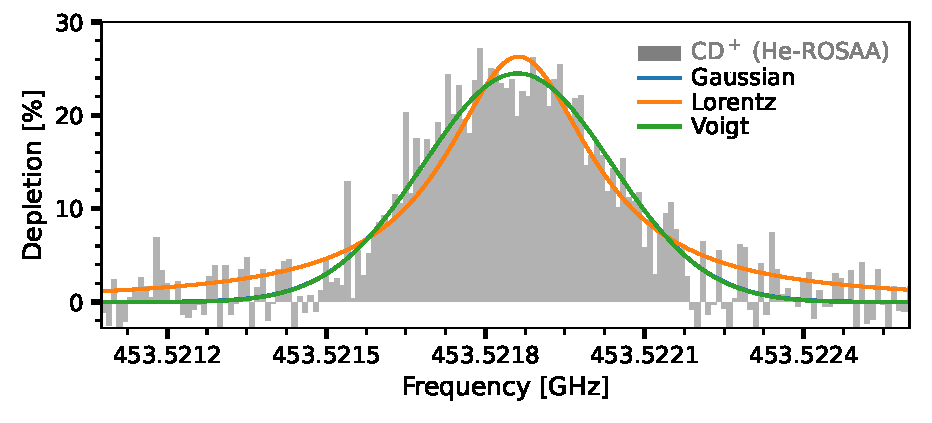
\includegraphics[width=1\textwidth]{figures/measurements/THz/thz_CD+_He.pdf}
%     \caption{\CD measured J$= 1-0$ rotational transition. The colored solid lines indicates the fitted line profile as labelled. The experiment performed at T$_{trap}=4.7(3)$K with He tag ROSAA technique (see Section \ref{subsec:ROSAA}) and derived T$_{ion} = 14(5)$K and T$_{coll} = 7(1)$K.}
%     \label{fig:thz:HeCD+}
% \end{figure}

% \begin{figure}
%     \centering
%     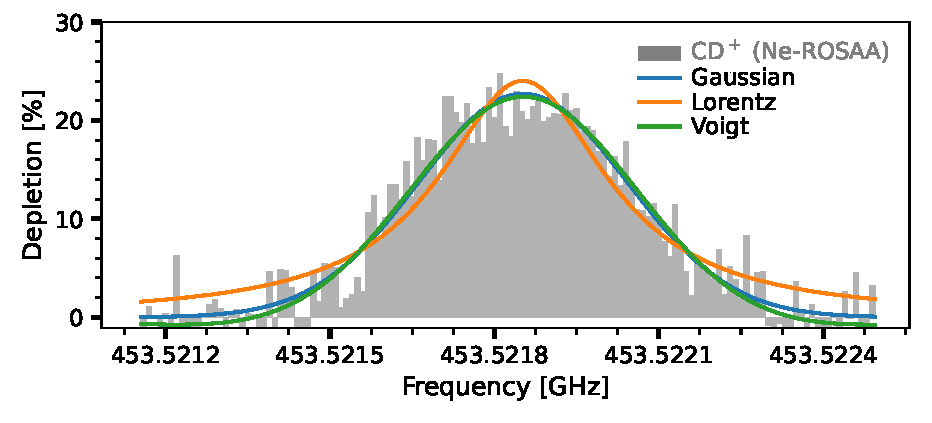
\includegraphics[width=1\textwidth]{figures/measurements/THz/thz_CD+_Ne.pdf}
%     \caption{\CD measured J$= 1-0$ rotational transition. The colored solid lines indicates the fitted line profile as labelled. The experiment performed at T$_{trap}=8.7(3)$K with He tag ROSAA technique (see Section \ref{subsec:ROSAA}) and derived T$_{ion} = 23(5)$K and T$_{coll} = 19(3)$K.}
%     \label{fig:thz:NeCD+}
% \end{figure}

\begin{figure}[!htb]
    \centering
    \begin{subfigure}[b]{0.49\textwidth}
        \centering
        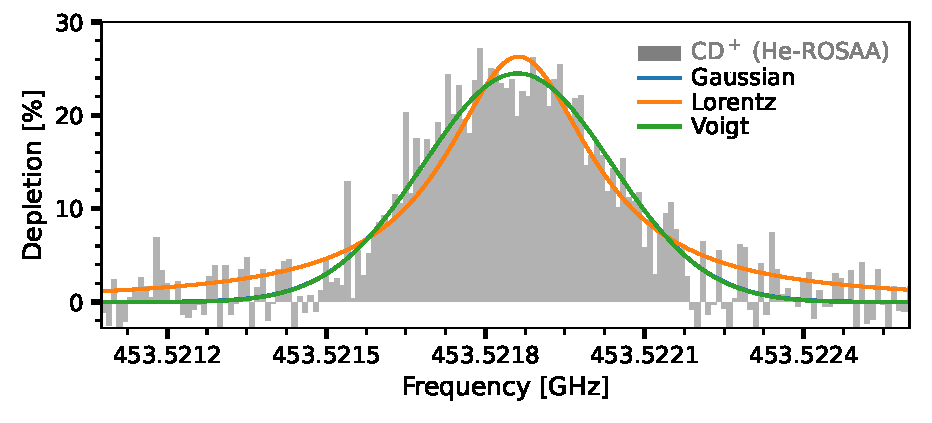
\includegraphics[width=1\textwidth]{figures/measurements/THz/thz_CD+_He.pdf}
        \caption{}
        \label{fig:thz:HeCD+}
    \end{subfigure}
    \hfill
    \begin{subfigure}[b]{0.49\textwidth}
        \centering
        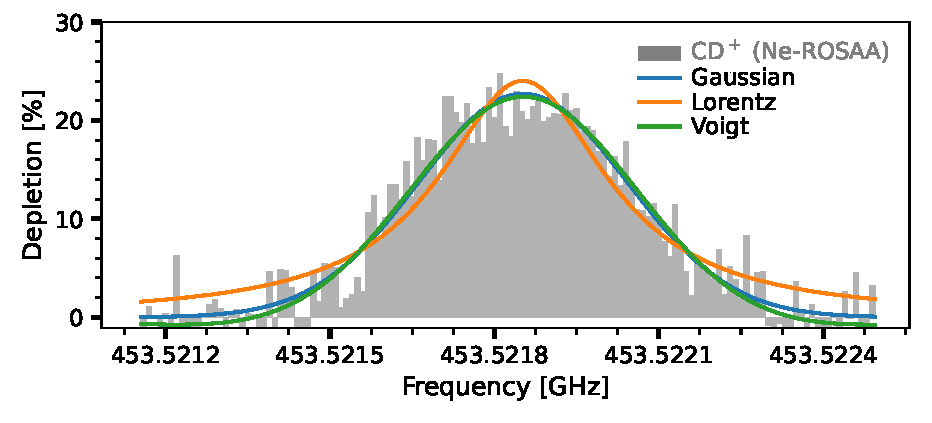
\includegraphics[width=1\textwidth]{figures/measurements/THz/thz_CD+_Ne.pdf}
        \caption{}
        \label{fig:thz:NeCD+}
    \end{subfigure}
    \caption{Measured \CD \CDline rotational transition using ROSAA technique  (see Section \ref{subsec:ROSAA}). The coloured solid lines indicate the fitted line profile as labelled. The experiment performed at $35(12) \mu$W power - (a) with He tag, T$_{trap}=4.7(3)$ K [He=$2.7(4) \cdot 10^{14}$ \percc] and derived T$_{ion} = 14(5)$ K and T$_{coll} = 7(1)$ K; (b) with Ne tag , T$_{trap}=8.7(3)$ K [Ne=$1.8(2)\cdot 10^{14}$ \percc] and derived T$_{ion} = 23(5)$ K and T$_{coll} = 19(3)$ K.}
    \label{fig:thz}
\end{figure}

% \begin{table}[!htb]
%     \centering
%     \caption{Pure-rotational \CDline transition frequency of \CD ion using ROSAA action spectroscopy with He tag at 4.5(3) and 5.6(2) K temperature, and $ 35 \sim \mu$W power.}
%     \begin{tabular}{rrrrr}
%         \hline                                                                       \\
%         T$_{trap}$ & Number density           & Frequency      & Depletion & FWHM    \\
%         K          & $\times 10 ^{14}$ \percc & MHz            & \%        & kHz     \\
%         \\\hline\hline\\
%         4.5(3)     & 2.2(3)                   & 453521.852(05) & 25.56(60) & 420(11) \\
%         4.5(3)     & 2.7(4)                   & 453521.856(05) & 24.79(61) & 406(12) \\
%         4.5(3)     & 5.7(7)                   & 453521.849(05) & 24.49(66) & 397(12) \\
%         5.6(2)     & 6.3(9)                   & 453521.849(13) & 13.19(90) & 384(30) \\
%         \\\hline\hline\\
%     \end{tabular}
%     \label{tab:CD+_He}
% \end{table}

Figure \ref{fig:thz} shows the measured \CD rotational spectrum using both He-
and Ne-attachment for the ROSAA method fitted with various lineshapes such as Gaussian,
Lorentz and Voigt. The experiment is repeated with various temperatures and
over large pressure ranges as summarized in Table \ref{tab:CD+_He} and
\ref{tab:CD+_Ne} with fitted parameters such as central transition frequency,
signal intensity (He\CD depletion \%) and full-width half maxima (FWHM). The
measured $J=0-1$ transition frequency fitted with a Voigt profile line shape is
453521.852(5) MHz via He-ROSAA and 453521.853(5) MHz via Ne-ROSAA,
respectively, and agrees well within the respective error bars with each other
and with the previous literature value 453521.8509(7) and 453521.8530(6) MHz
via He-ROSAA by \citet{Brunken2017} and \citet{domenech_first_2018},
respectively, and with an earlier absorption study in a glow discharge experiment 453521.851(20) MHz by
\citet{amano_j_2010}.


% \begin{figure}
%     \centering
%     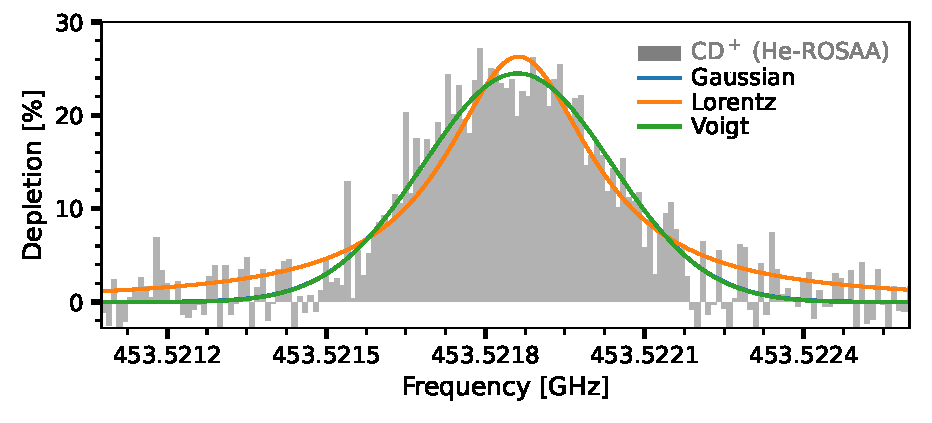
\includegraphics[width=1\textwidth]{figures/measurements/THz/thz_CD+_He.pdf}
%     \caption{\CD measured J$= 1-0$ rotational transition. The colored solid lines indicates the fitted line profile as labelled. The experiment performed at T$_{trap}=4.7(3)$K with He tag ROSAA technique (see Section \ref{subsec:ROSAA}) and derived T$_{ion} = 14(5)$K and T$_{coll} = 7(1)$K.}
%     \label{fig:thz:HeCD+}
% \end{figure}

% \begin{figure}
%     \centering
%     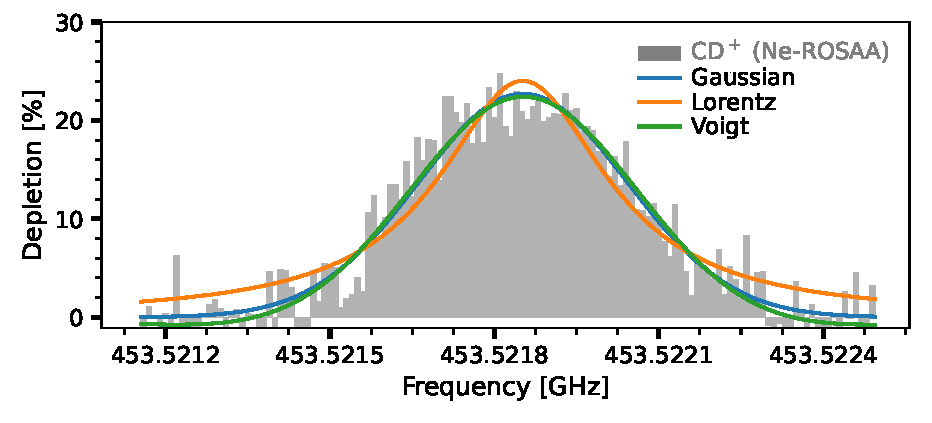
\includegraphics[width=1\textwidth]{figures/measurements/THz/thz_CD+_Ne.pdf}
%     \caption{\CD measured J$= 1-0$ rotational transition. The colored solid lines indicates the fitted line profile as labelled. The experiment performed at T$_{trap}=8.7(3)$K with He tag ROSAA technique (see Section \ref{subsec:ROSAA}) and derived T$_{ion} = 23(5)$K and T$_{coll} = 19(3)$K.}
%     \label{fig:thz:NeCD+}
% \end{figure}

\begin{figure}[!htb]
    \centering
    \begin{subfigure}[b]{0.49\textwidth}
        \centering
        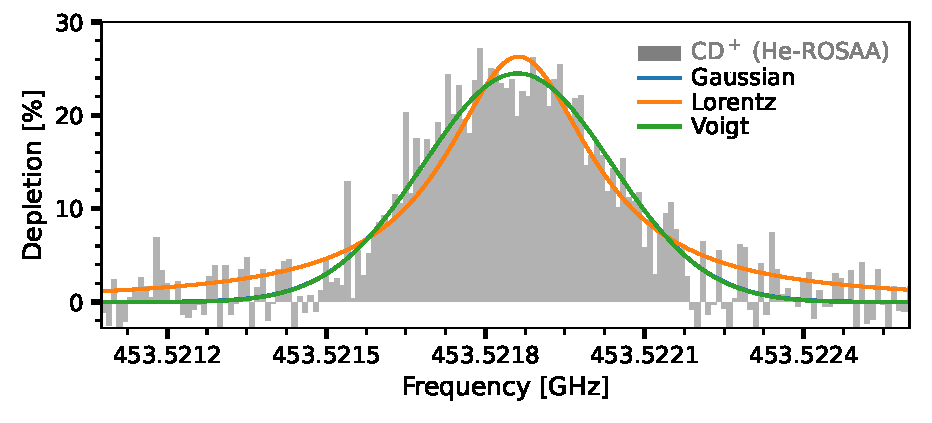
\includegraphics[width=1\textwidth]{figures/measurements/THz/thz_CD+_He.pdf}
        \caption{}
        \label{fig:thz:HeCD+}
    \end{subfigure}
    \hfill
    \begin{subfigure}[b]{0.49\textwidth}
        \centering
        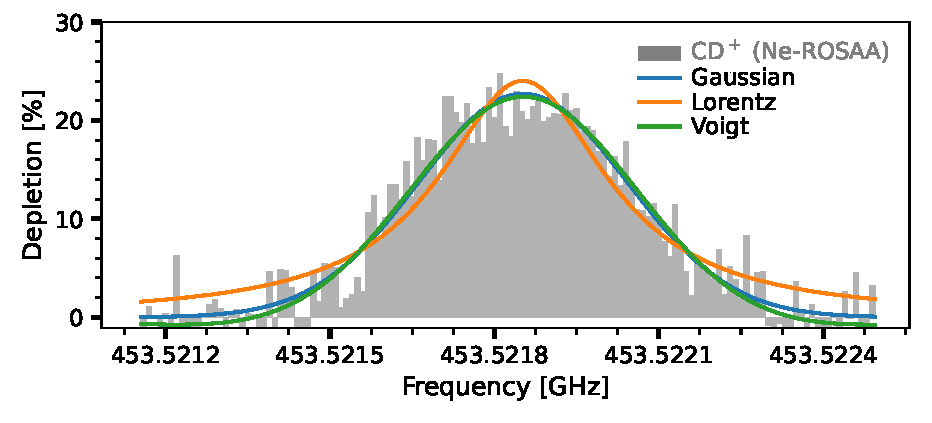
\includegraphics[width=1\textwidth]{figures/measurements/THz/thz_CD+_Ne.pdf}
        \caption{}
        \label{fig:thz:NeCD+}
    \end{subfigure}
    \caption{Measured \CD \CDline rotational transition using ROSAA technique  (see Section \ref{subsec:ROSAA}). The coloured solid lines indicate the fitted line profile as labelled. The experiment performed at $35(12) \mu$W power - (a) with He tag, T$_{trap}=4.7(3)$ K [He=$2.7(4) \cdot 10^{14}$ \percc] and derived T$_{ion} = 14(5)$ K and T$_{coll} = 7(1)$ K; (b) with Ne tag , T$_{trap}=8.7(3)$ K [Ne=$1.8(2)\cdot 10^{14}$ \percc] and derived T$_{ion} = 23(5)$ K and T$_{coll} = 19(3)$ K.}
    \label{fig:thz}
\end{figure}

\begin{table}[!htb]
    \centering
    \caption{Pure-rotational \CDline transition frequency of \CD ion using ROSAA action spectroscopy with He tag at 4.5(3) and 5.6(2) K temperature, and $ 35 \sim \mu$W power.}
    \begin{tabular}{rrrrr}
        \hline                                                                       \\
        T$_{trap}$ & Number density           & Frequency      & Depletion & FWHM    \\
        K          & $\times 10 ^{14}$ \percc & MHz            & \%        & kHz     \\
        \\\hline\hline\\
        4.5(3)     & 2.2(3)                   & 453521.852(05) & 25.56(60) & 420(11) \\
        4.5(3)     & 2.7(4)                   & 453521.856(05) & 24.79(61) & 406(12) \\
        4.5(3)     & 5.7(7)                   & 453521.849(05) & 24.49(66) & 397(12) \\
        5.6(2)     & 6.3(9)                   & 453521.849(13) & 13.19(90) & 384(30) \\
        \\\hline\hline\\
    \end{tabular}
    \label{tab:CD+_He}
\end{table}

% \begin{table}[!htb]
    \centering
    \caption{Pure-rotational \CDline transition frequency of \CD ion using ROSAA action spectroscopy with He tag at 4.5(3) and 5.6(2) K temperature, and $35 \sim \mu$W power.}
    \begin{tabular}{rrrrr}
        \hline\\
        T$_{trap}$ & Number density & Frequency & Depletion & FWHM \\
        K & $\times 10 ^{14}$ \percc & MHz & \% & kHz \\
        \\\hline\hline\\
        4.5(3)	& 2.2(3) & 453521.852(05)   & 25.56(60)	& 420(11) \\
        4.5(3)	& 2.7(4) & 453521.856(05)   & 24.79(61)	& 406(12) \\
        4.5(3)	& 5.7(7) & 453521.849(05)   & 24.49(66)	& 397(12) \\
        5.6(2)	& 6.3(9) & 453521.849(13)   & 13.19(90)	& 384(30) \\
        \\\hline\hline\\
    \end{tabular}
    \label{tab:CD+_He}
\end{table}

\begin{table}[!htb]
    \centering
    \caption{Pure-rotational \CDline transition frequency of \CD ion using ROSAA action spectroscopy with Ne tag for temperature range 5-14 K, and $35 \sim \mu$W power.}
    \begin{tabular}{rrrrr}
        \hline\\
        T$_{trap}$ & Number density & Frequency & Depletion & FWHM \\
        K & $\times 10 ^{14}$ \percc & MHz & \% & kHz \\
        \\\hline\hline\\
        16	& 1.9(2)    & 453521.908(35) & 	11(2) & 455(083) \\
        16	& 1.9(2)    & 453521.845(63) & 	06(1) & 563(148) \\
        14	& 1.5(2)    & 453521.872(26) & 	14(1) & 610(060) \\
        8,7	& 1.2(2)    & 453521.843(33) & 	19(4) & 355(078) \\
        8,7	& 1.8(2)    & 453521.848(06) & 	22(1) & 446(014) \\
        8,7	& 1.5(2)    & 453521.847(09) & 	24(1) & 448(022) \\
        9	& 3.8(5)    & 453521.828(26) & 	14(3) & 253(060) \\
        9	& 2.0(3)    & 453521.858(09) & 	19(1) & 390(021) \\
        5,5	& 8(1)	    & 453521.852(26) & 	12(3) & 204(061) \\
        6	& 1.0(1)    & 453521.845(28) & 	19(2) & 414(065) \\
        \\\hline\hline\\
    \end{tabular}

    \label{tab:CD+_Ne}
\end{table}
\begin{table}[!htb]
    \centering
    \caption{Pure-rotational \CDline transition frequency of \CD ion using ROSAA action spectroscopy with Ne tag for temperature range 5-14 K and $35 \sim \mu$W power.}
    \begin{tabular}{rrrrr}
        \hline                                                                        \\
        T$_{trap}$ & Number density           & Frequency      & Depletion & FWHM     \\
        K          & $\times 10 ^{14}$ \percc & MHz            & \%        & kHz      \\
        \\\hline\hline\\
        16         & 1.9(2)                   & 453521.908(35) & 11(2)     & 455(83) \\
        16         & 1.9(2)                   & 453521.845(63) & 6(1)      & 563(148) \\
        14         & 1.5(2)                   & 453521.872(26) & 14(1)     & 610(60) \\
        8.7        & 1.2(2)                   & 453521.843(33) & 19(4)     & 355(78) \\
        8.7        & 1.8(2)                   & 453521.848(6)  & 22(1)     & 446(14) \\
        8.7        & 1.5(2)                   & 453521.847(9)  & 24(1)     & 448(22) \\
        9          & 3.8(5)                   & 453521.828(26) & 14(3)     & 253(60) \\
        9          & 2.0(3)                   & 453521.858(9)  & 19(1)     & 390(21) \\
        5.5        & 8(1)                     & 453521.852(26) & 12(3)     & 204(61) \\
        6          & 1.0(1)                   & 453521.845(28) & 19(2)     & 414(65) \\
        \\\hline\hline\\
    \end{tabular}

    \label{tab:CD+_Ne}
\end{table}

\clearpage

\subsection{Determining ion temperature}
\label{subsec:CD+-Tion}

The ion temperature (T$_{ion}$) can be determined from a measured line profile
fitted with a Voigt lineshape (see Section
\ref{subsec:collisional-ion-temperature} for detail). Figure \ref{fig:Tcoll}
shows the plot comparing measured nominal trap temperature, T$_{trap}$ and
derived T$_{ion}$ for \CD from Table \ref{tab:CD+_He} and \ref{tab:CD+_Ne}.
The plot is compared with the previously determined values in the FELion
instrument by \citet{kluge_state-selective_2016}. This confirms that the ion
temperature is higher than the nominal trap temperatures, as observed
previously in the 22-pole ion trap \cite{asvany_numerical_2009, otto_internal_2013, endres_incomplete_2017}. 
For T$_{trap} < 5$ and $>5$ K, the corresponding T$_{ion}$ are derived from He-ROSAA and Ne-ROSAA
measurements, respectively. Each data points in Figure \ref{fig:Tcoll} is an averaged value
of corresponding T$_{ion}$ derived from atleast two measurements of FWHM as shown in Table \ref{tab:CD+_He} 
and \ref{tab:CD+_Ne}. The large uncertainty of T$_{ion}$ value in our measurement is because of the
large uncertainty in the derived FWHM from measured line profile (see Table \ref{tab:CD+_He} and \ref{tab:CD+_Ne}).
However, the trend of T$_{ion}$ with T$_{trap}$ is consistent with the previous measurements.

\begin{figure}[!htb]
    \centering
    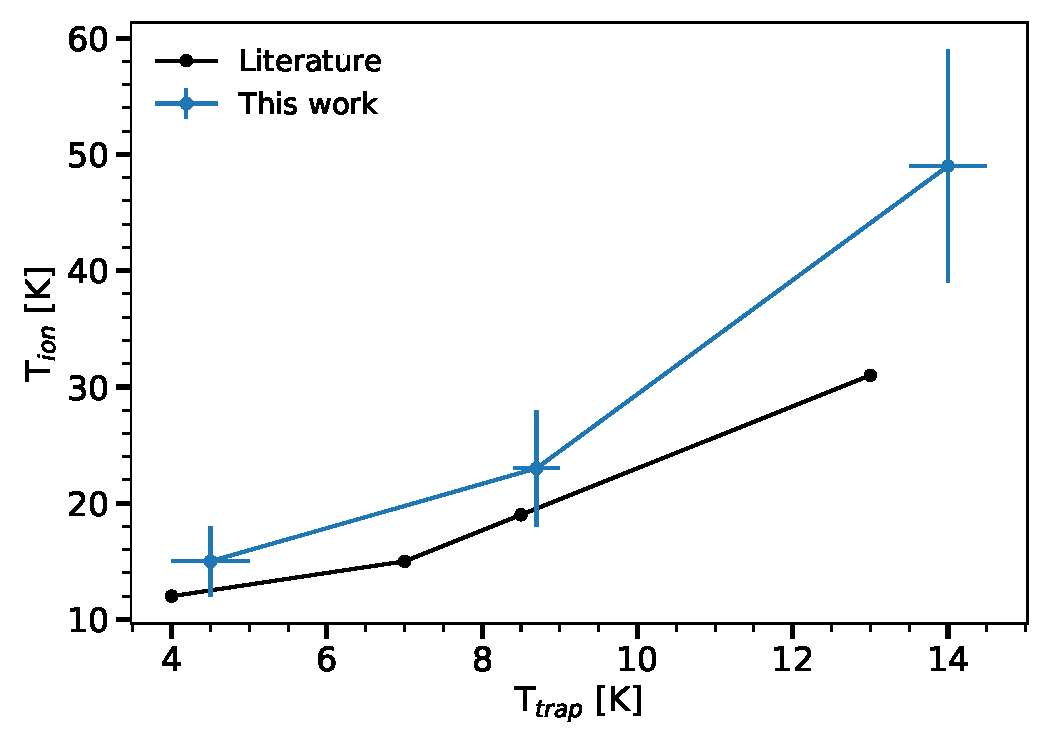
\includegraphics[scale=0.5]{figures/measurements/THz/CD+_Tcoll.pdf}
    \caption{Comparing nominal trap temperature (T$_{trap}$) and ion temperature (T$_{ion}$) derived from the rotational spectrum. The solid (black) line corresponds to Ref. \cite{kluge_state-selective_2016}, and the solid (\textcolor{blue}{blue}) represents data in this work (see text).}
    \label{fig:Tcoll}
\end{figure}
Our measured \Tion data lies higher than the previous literature data (see Figure \ref{fig:Tcoll}). However, different experimental conditions could explain this difference. Since, as discussed by \citet{endres_incomplete_2017}, various factors such as RF heating, buffer gas thermalisation with trap walls, black-body radiation from surrounding room temperature vacuum chamber, and collision with warm residual gas that enter the cryogenic trap, in principle, can influence the ion temperature.

% The measurements are performed at $\sim 35\ \mu$W for \CD $J=0-1$ transition.
% Similar to deriving T$_{ion}$, one could also derive the power from the Lorentzian parameters using equation \ref{eqn:fL}. However, as depicted in Figure \ref{fig:thz}, the Gaussian part dominates and, thus, the Lorentzian parameters and, subsequently, the power could not be determined within reasonable error limits.
% maybe include this in the discussion later ?
% The \Tion dependency for \CD on the ion-to-buffer gas mass ratio, i.e., for He
% and Ne, could not be determined in this study. However,
% \citet{endres_incomplete_2017} showed that for OH$^-$, \Tion is independent
% of the ion-to-buffer gas mass ratio using He and HD. 
The number density variation in the range $(2-6) \cdot 10^{14}$ \percc\ around 5 K temperature
for helium (see Table \ref{tab:CD+_He}) did not influence the derived T$_{ion}$
within the error limits. The effective collisional temperature, i.e., T$_{coll}$, is derived from \Ttrap
and \Tion using equation \ref{eqn:Tcoll}. In detail, the following sections
investigate the kinetic measurement in the presence of radiation and ROSAA
simulations at a given collisional temperature.


\subsection{Kinetics}
\label{subsec:CD+-kinetics}

The measured formation rate constants ($k_3$) in kinetic experiments are 
weighted average rate coefficients over the thermal population of rotational
levels ($J$) at a given collisional temperature (T$_{coll}$). The rotational
state-specific ternary rate constants ($k_{3_1}$) for the first attachment process can be written as:
\begin{equation}
    k_{3_1} (T_{coll}) = \frac{\sum_{J} k_{3_1} (J, \text{T}_{coll}) \cdot N_{\text{CD}^+ (J)} }{N_{\text{CD}^+}}
    \label{eqn:rate-constant-weighted}
\end{equation}

where $N_{\text{CD}^+ (J)}$ indicate the thermal population at a specific rotational $J$ level 
and $N_{\text{CD}^+}$ is the total population of \CD ion on all $J$ levels.\\

\begin{figure}[!htb]
    \centering
    \begin{subfigure}[b]{0.49\textwidth}
        \centering
        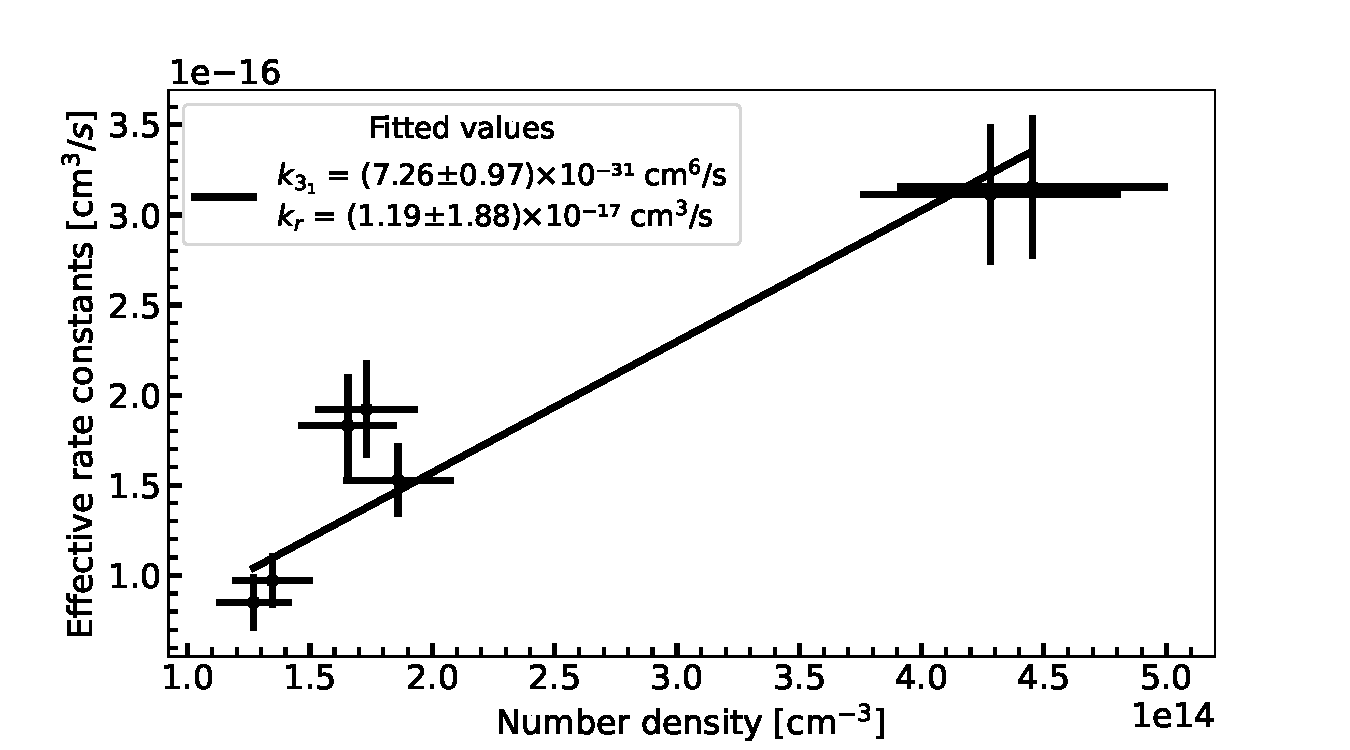
\includegraphics[width=1\textwidth]{figures/measurements/kinetics/functionOf_nHe/on_4.8K_k31_effective_rate_constants.pdf}
        \caption{}
        \label{fig:on:effective-rate-constants}
    \end{subfigure}
    \hfill
    \begin{subfigure}[b]{0.49\textwidth}
        \centering
        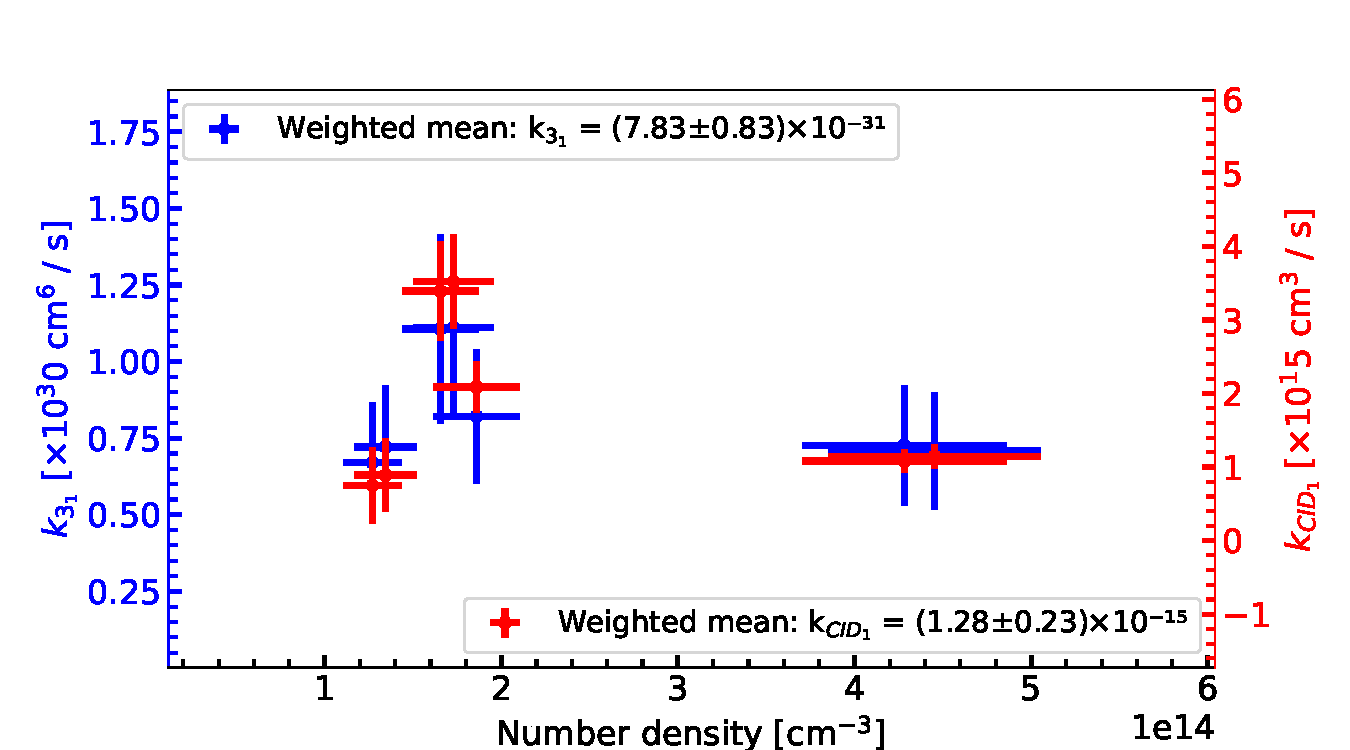
\includegraphics[width=1\textwidth]{figures/measurements/kinetics/functionOf_nHe/on_4.8K_k3_kCID_1_as_functionOfnHe.pdf}
        \caption{}
        \label{fig:on:rate-constants}
    \end{subfigure}

    \caption{Deriving rate coefficients in the presence of radiation resonant with the $J=0-1$ transition of \CD. (a) The effective binary rate constant ($k_e$) is plotted as a function of number density to derive $k_{3_1}$ (ternary association) and $k_r$ (radiative) rate constants. The solid line indicates the linear fit where the slope and intercept correspond to $k_3$ and $k_r$, respectively. (b) shows the ternary association (\textcolor{blue}{$k_{3_1}$}) and collision-induced dissociation (\textcolor{red}{$k_{CID_1}$}) rate constants plotted as a function of helium number density under the assumption: $k_3[He] \gg k_r$(see text). The weighted mean values are shown in the legend box.}
    \label{fig:on:effective-and-ternary}

\end{figure}

Figure \ref{fig:on:effective-and-ternary} shows the He\CD formation rate
coefficient as described in equation \ref{eqn:rate-constant-weighted}. The
formation rate coefficients ($k_{3_1}$) for the first complex (He\CD) measured with and without the presence of radiation resonant with the $J=0-1$ transition of \CD ion is denoted by $k_{3_1}(ON)$ and
$k_{3_1}(OFF)$, respectively (see Figure \ref{fig:off:rate-constants} and \ref{fig:on:rate-constants}).

The derived rate constants at T$_{coll}=7$ K and P$=3.5\times 10^{-5}$ W, is given by:
\begin{align}
    \label{eqn:k-on-off}
    \begin{split}
        k_{3_1}(OFF) &= 1.1(1) \cdot 10^{-30} \text{ cm}^6/\text{s}\\
        k_{3_1}(ON) &= 7.8(8) \cdot 10^{-31} \text{ cm}^6/\text{s}
    \end{split}
\end{align}

Following the discussion from Section \ref{subsec:ROSAA-simulation}, the
state-dependent formation rate constant is the key factor in understanding the
ROSAA process and, subsequently, its signal intensity (referred to as depletion
counts [\%] in Figure \ref{fig:thz}). The next section discusses this
relationship in detail with numerical simulations.

\section{ROSAA Numerical simulation}
\label{subsec:CD+-kinetics-simulation}

In this section, we shall discuss the results from the numerical simulation of
the ROSAA processes described in detail in Section
\ref{subsec:ROSAA-simulation}.

\subsection{Collisional process}
\label{subsec:CD+-kinetics-simulation-coll}

As the hot \CD ions from the ion source (T$_{coll}=300$ K) enter the 22-pole
ion trap (T$_{trap}=4.8(3)$ K), they are collisionally cooled down by He buffer
gas atoms and, at equilibrium, reach the effective collision temperature
(T$_{coll}=7(1)$ K). The T$_{coll}$ is derived using T$_{ion}$ and T$_{trap}$
temperature as described in Eq. \ref{eqn:Tcoll} (see Section
\ref{subsec:CD+-Tion}). In the absence of radiation and attachment processes,
the collisional process reaches an equilibrium of the relative population of
rotational quantum states, which is given by the Boltzmann distribution (at
\Tcoll), as shown in Figure
\ref{fig:ROSAA-sim-collisional-boltzman-comparision} (see Section
\ref{subsec:ROSAA-simulation-coll}). The collisional rate coefficient values
are derived from \citet{Werfelli2017}, for T$_{coll}=7$ K, the rate constants
for $J=0-5$ are given in Appendix Table
\ref{appendix:tab:collisional-rate-coefficients}. The rates are in the order of
$>10^4$ \pers\ for $2.2 \cdot 10^{14}$ \percc\ helium number density. As can be
seen in Fig. \ref{fig:ROSAA-sim-collisional-boltzman-comparision},
thermalization of the initially hot ions to the Boltzmann distribution at the
collisional temperature happens within 0.3 ms under typical experimental
conditions.

\begin{figure}[!htb]
    \Subfigure[0.49]{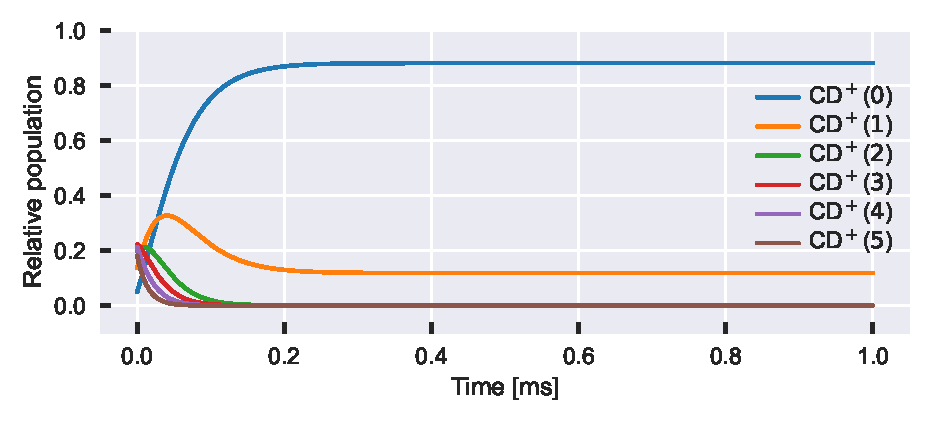
\includegraphics[width=1\textwidth]{figures/simulations/collisional/CD+_He_f-time__transition_0-1_0.001s_population_ratio.pdf}}{}{\label{fig:ROSAA-sim-collisional}}
    \hfill
    \Subfigure[0.49]{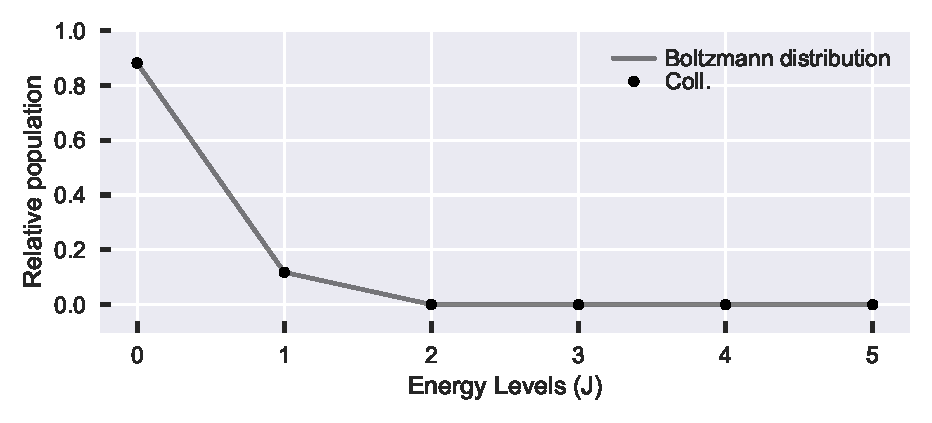
\includegraphics[width=1\textwidth]{figures/simulations/collisional/CD+_He_f-time__transition_0-1_0.001s_boltzman_comparision.pdf}}{}{\label{fig:ROSAA-sim-collisional-boltzmann}}
    \caption{(a) Collisional process for \CD ions up to $J=5$ with He buffer gas ([He]$=2.2 \cdot 10^{14}$ \percc). The 
    coloured label indicates the corresponding \CD$(J)$ state. At $t=0$, the relative population
    corresponds to a Boltzmann distribution at T$_{coll}=300$ K. The relative population evolves through collisions 
    with He with rate constants for T$_{coll}=7$ K (derived from \cite{Werfelli2017}), subsequently reaching 
    equilibrium after $<0.5$ ms. (b) Comparison of the Boltzmann distribution at 7 K with the relative population 
    involving only collisional process (Coll.) at $t=1$ ms.}
    \label{fig:ROSAA-sim-collisional-boltzman-comparision}
\end{figure}
The spontaneous emission rates $(A)$ are also included in this process, as discussed in section \ref{subsec:ROSAA-simulation-spont}. However, the collision process dominates it by $8$ orders of magnitude (see Table \ref{appendix:tab:collisional-rate-coefficients} and \ref{appendix:tab:radiative-rate-coefficients}). Therefore, in the following sections, spontaneous emission rates will not be mentioned specifically, although it is included in all the cases during simulation.

\subsection{Radiative processes}
\label{subsec:CD+-kinetics-simulation-coll-rad}

As discussed above, when including only the collisional process, the relative
population re-distributed from room temperature (300 K) to a Boltzmann
distribution (T$_{coll}=7$ K) at equilibrium within $<0.5$ ms. Furthermore, in
the presence of radiation resonant with $J=0-1$ of \CD, the population can be
further re-distributed due to a competing radiative process as shown in Figure
\ref{fig:ROSAA-sim-coll-rad-population-boltzmann}. The simulation of the
evolution of the relative population of the \CD$(J)$ rotational levels is shown
in Figure \ref{fig:ROSAA-sim-coll-rad-population} for a duration of 1 ms. The
derivation of radiative rates is described in detail in section
\ref{subsec:ROSAA-simulation-rad}. The radiative rates for a radiation power $35\ \mu$W are
in the same order of magnitude as collisional rates, i.e., $>10^{4}$ \pers\
(see Table \ref{appendix:tab:radiative-rate-coefficients}).

\begin{figure}[!htb]
    % \centering
    \Subfigure[0.49]{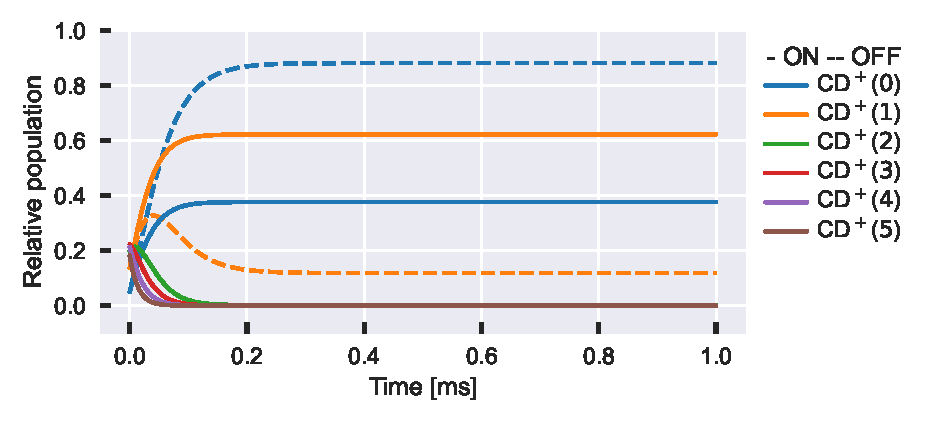
\includegraphics[width=1\textwidth]{figures/simulations/coll_rad/CD+_He_f-time__transition_0-1_0.001s_population_ratio.pdf}}{}{\label{fig:ROSAA-sim-coll-rad-population}}
    \hfill
    \Subfigure[0.49]{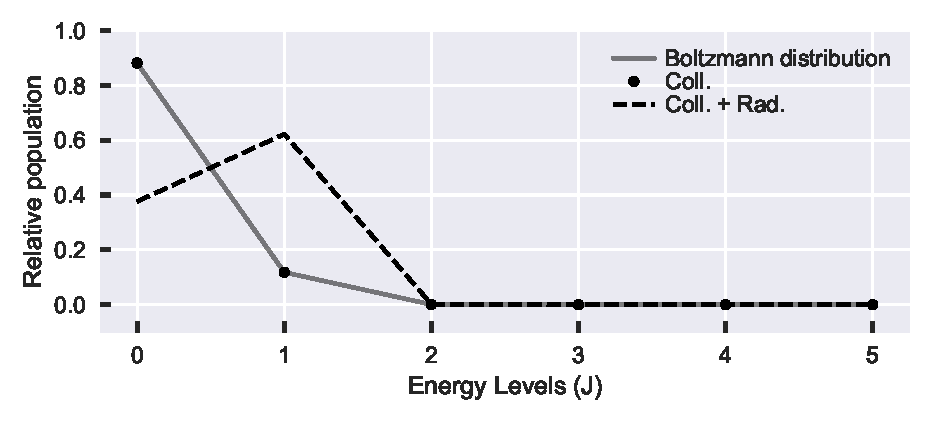
\includegraphics[width=1\textwidth]{figures/simulations/coll_rad/CD+_He_f-time__transition_0-1_0.001s_boltzman_comparision.pdf}}{}{\label{fig:ROSAA-sim-coll-rad-boltzmann}}
    
    \caption{(a) Simulated relative rotational level populations for \CD as labelled in parenthesis. The population evolves from $t=0$ (T$_{coll}=300$ K) to reach equilibrium at $t<0.5$ ms. The solid and dashed lineshapes correspond with (ON) and without (OFF) the presence of radiation on the \CD \CDline transition. The radiation power is $35\ \mu$ W. (b) Comparison of the Boltzmann distribution at 7 K with the relative population involving only collisional process (Coll.) and, collision and radiative process (Coll. + Rad.) at $t=1$ ms.}
    \label{fig:ROSAA-sim-coll-rad-population-boltzmann}
\end{figure}


As depicted in Figure \ref{fig:ROSAA-sim-coll-rad-boltzmann}, the distribution
no longer follows a Boltzmann distribution. Furthermore, if the radiative rates
dominate the collisional rates (Coll. $\ll$ Rad), say for power $10^{5}$
higher, i.e., 3.5 W, we get rates in the order of $>10^{7}$ \pers. The
resulting population on $J=0$ and $J=1$ quantum levels should then reach their
statistical weights ($g(J) = 2J + 1$). The simulated relative population
evolution and equilibrium population under the condition Coll. $\ll$ Rad. is
shown in Figure \ref{fig:ROSAA-sim-coll-rad-population-boltzmann-higher-rad},
for a duration of 1 ms. Figure
\ref{fig:ROSAA-sim-coll-rad-boltzmann-higher-rad} also clearly shows the $J=0$
and $J=1$ rotational states reaching their statistical weight of 0.25 and 0.75,
respectively.

\begin{figure}[!htb]
    % \centering
    \Subfigure[0.49]{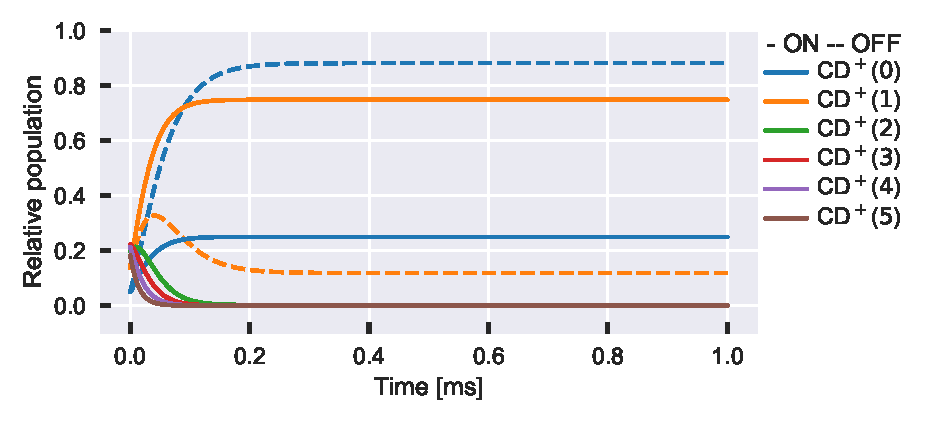
\includegraphics[width=1\textwidth]{figures/simulations/coll_rad/CD+_He_f-time__transition_0-1_0.001s_population_ratio-higher-rad.pdf}}{}{\label{fig:ROSAA-sim-coll-rad-population-higher-rad}}
    \hfill
    \Subfigure[0.49]{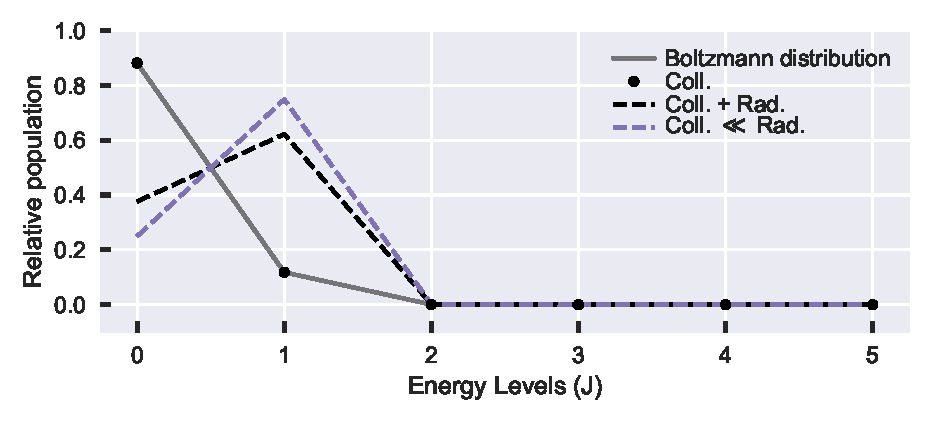
\includegraphics[width=1\textwidth]{figures/simulations/coll_rad/CD+_He_f-time__transition_0-1_0.001s_boltzman_comparision-higher-rad.pdf}}{}{\label{fig:ROSAA-sim-coll-rad-boltzmann-higher-rad}}
    
    \caption{(a) Simulated relative rotational level populations for \CD and corresponding number $J$ levels as labelled in parenthesis. The population evolves from $t=0$ (T$_{coll}=300$ K) to reach equilibrium at $t<0.5$ ms. The solid and dashed lineshapes correspond with (ON) and without (OFF) the presence of radiation on the \CD \CDline transition. The radiation power is 3.5 W. (b) Compares the Boltzmann distribution at 7 K with the relative population involving only collisional process (Coll.), collision and radiative process for power $3.5\ \mu$W (Coll. + Rad.), and collision and radiative process for power 3.5 W (Coll. $\ll$ Rad.), at $t=1$ ms.}
    \label{fig:ROSAA-sim-coll-rad-population-boltzmann-higher-rad}
\end{figure}

The next section investigates the helium attachment process, vital in
understanding the ROSAA signal, i.e., the measured peak intensity [in $\%$].

\subsection{Attachment processes}
\label{subsec:CD+-kinetics-simulation-coll-rad-att}

As the \CD ions collide with the He buffer gas at low temperature and high
number density, they form He complexes, i.e., He$_n$\CD. The formation and
subsequent dissociation rate coefficients of He$_n$\CD are discussed in section
\ref{subsec:rate-constants}. The numerical simulation method for the attachment
process is described in detail in Section \ref{subsec:ROSAA-simulation-att}.

The ROSAA action spectroscopic technique utilises the rotation-specific
rate coefficients for the helium attachment process to observe a change in
helium-complexes formed at resonant frequency (see Section
\ref{sec:methods:rotation}). Since, as discussed above, involving radiative
processes re-distributes the population of rotational quantum states this
subsequently results in different numbers of complexes formed, thus a
ROSAA-signal, i.e., depletion counts [\%] of He\CD as shown in Figure
\ref{fig:thz:HeCD+}.

A complete simulation involving the radiation, collisional, and attachment
processes is vital to investigate the experimentally measured rotational
spectrum, i.e., ROSAA-signal intensity. However, a rotational state-specific
rate coefficient is required to include the attachment process, which is not
straightforward to measure directly. Nevertheless, as discussed in section
\ref{sec:CD+-kinetics}, a weighted rate coefficient was measured for the \CD + He 
reaction, with and without the presence of radiation resonant with
the $J=0-1$ transition of the \CD ion, and this allows to obtain the ratio between the
rate-coefficients in the two rotational levels.

Since the relative population of ${\text{CD}^+}(0) + \text{CD}^+(1) \geq 0.97 $
at T$_{coll}=7$ K (see Figure \ref{fig:ROSAA-sim-collisional}), we can assume a
2-level quantum system to determine the rotational state-specific ternary rate
constants ($k_{3_1}(J)$) from the measured, weighted ternary rate coefficients
($k_{3_1}$) using Equation \ref{eqn:rate-constant-weighted}. The $k_{3_1}$
ratio (also referred to as \qt{$a$}) is given by:

\begin{equation}
    \begin{split}
        a & = \frac{k_{3_1}(J=1)}{k_{3_1}(J=0)}\\
        & = \frac{X \cdot \text{CD}^+(0) - \text{CD}^+(0)_{on}}{\text{CD}^+(1)_{on} - X\cdot \text{CD}^+(1)}
    \end{split}
    \label{eqns:rate-constant-change-ratio}
\end{equation}

where $X$ is the ratio of measured weighted rate constant with (ON) and without
(OFF) radiation, i.e., $X=k_{3_1}(ON) / k_{3_1}(OFF)$, and \CD$(0)$ and \CD$(1)$
represents \CD rotational population ratio at $J=0$ and $J=1$, respectively.
The subscript $on$ indicates the relative population in the presence of
radiation; otherwise no radiation was admitted.\\

Using $k_{3_1}(ON)$ and $k_{3_1}(OFF)$ value from equation \ref{eqn:k-on-off},
we get $X$ as:

\begin{equation}
    X = 0.7(1)
    \label{eqn:derived-X-value}
\end{equation}

and for the following conditions \footnote{\textit{refer Section
        \ref{subsec:rot:power} for power derivation, Section
        \ref{subsec:collisional-ion-temperature} and Figure \ref{eqn:Tcoll} for
        T$_{coll}$ derivation}},

\begin{align*}
    T_{coll} & = 7\ \text{K}                      \\
    [He]     & = 2.2 \cdot 10^{14}\ \text{\percc} \\
    P        & = 3.5 \cdot 10^{-5}\ \text{W}
\end{align*}

the relative population for \CD$(J)$ is given as (see Figure
\ref{fig:ROSAA-sim-collisional} and \ref{fig:ROSAA-sim-coll-rad-population}):

\begin{align}
    \cd^+(0)      & = 0.9                                  \\
    \cd^+(1)      & = 0.1                                  \\
    \cd^+(0)_{on} & = 0.4                                  \\
    \cd^+(1)_{on} & = 0.6 \label{eqn:CD+-population-value}
\end{align}

Substituting equations \ref{eqn:derived-X-value} through
\ref{eqn:CD+-population-value} in Eq. \ref{eqns:rate-constant-change-ratio}, we
can get an experimentally derived $k_{3_1}$ ratio as:

\begin{equation}
    a = 0.5(2)
    \label{eqn:k31-ratio}
\end{equation}

The derived $k_{3_1}$ ratio value, $a=0.5(2)$, agrees within the uncertainties of the previously
estimated value $a=0.55(5)$ from \citet{Brunken2017}. In the previous study,
\cite{Brunken2017}, the \qt{$a$} value is estimated by measuring the \CDline
transition of \CD at different number density and radiation power and fitting
the measured ROSAA depletion signal intensity to the numerical model. However,
in this study, the \qt{$a$} is experimentally derived from kinetic measurement
in the presence and absence of radiation resonant with \CDline of \CD molecular
ion. This approach also directly validates equation
\ref{eqn:rate-constant-weighted}, and thereby, the rotational state-dependent
attachment of rare gas atoms to molecular ions. In addition, this
systematically supports our investigation of various processes involved in the
ROSAA technique. As described in Section \ref{sec:CD+-kinetics-motivation},
the main motivation is to develop a robust general-purpose ROSAA numerical
model that is adaptable to systematically add various processes.

In the following section, the derived \qt{$a$} is used to analyse the full
model, including collisional, radiation and attachment process to the measured
pure rotational transition intensity of the \CD ion.

\subsection{Analysing numerical results}
\label{subsec:CD+-kinetics-simulation-analysis}

The full model simulation, i.e., including collisional, radiation and
attachment processes for the \CD molecular ion up to 5 rotational quantum states
($J=0-5$), is shown in Figure \ref{fig:thz-sim:rel-pop:1ms} for T$_{coll}=7$ K
temperature, $2.2 \cdot 10^{14}$ \percc\ helium number density, $k_{3_1}$
ratio, $a=0.5$ and $3.5\ \mu$W power.
% In addition to \CD, the simulation considers up to two complexes (He\CD and He$_2$\CD) at 7 K temperature, $2.2 \cdot 10^{14}$ \percc\ helium number density, $k_{3_1}$ ratio, $a=0.5$ and $3.5\ \mu$W power. 
The \CD$(J)$ level with $J>3$ become insignificantly populated within $<0.5$ ms, i.e.,
reaching $\ll 10^{-10}$ in relative population ratio while \CD(2) and \CD(3)
equilibrate to $<10^{-2}$ and $<10^{-6}$, respectively, in relative population. 
Therefore, in this simulation the ternary attachment rate coefficients $k_{3_1}(J\geq 2)=0$
due to insignificant population in these states. Consequently, only the
\CD$(J=0)$ and \CD$(J=1)$ participate in the cluster formation. However, the
\CD$(J \geq 2)$ is included in the simulation to monitor its relative
population evolution.

% \begin{figure}
    \centering
    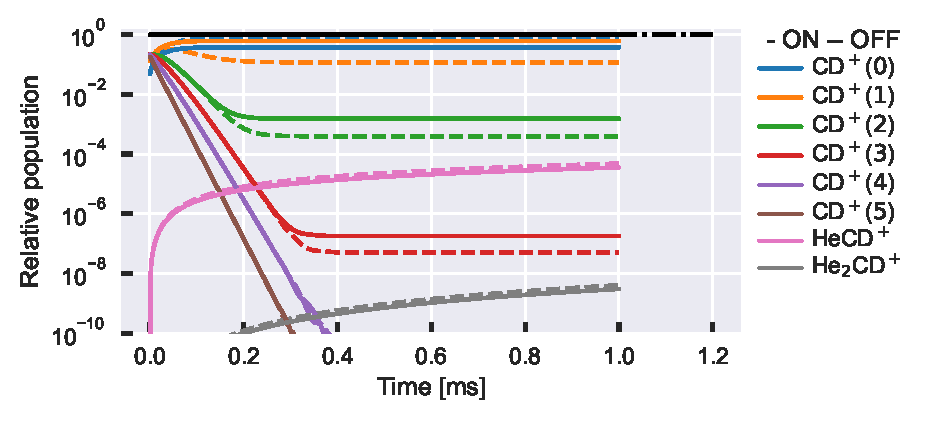
\includegraphics[width=1\textwidth]{figures/simulations/coll_rad_att/CD+_He_f-time__transition_0-1_0.001s_population_ratio.pdf}
    \caption{Simulated relative rotational level populations for \CD and corresponding number He$_n$\CD clusters (n=1, 2) as labelled in (top right) and \CD$(J)$ indicates \CD in $J$ rotational state. The simulation conditions are as follows: $k_{3_1}$ ratio, $a=0.5$, collisional rates for T$_{coll}=7$ K  (at $t=0$, T$_{coll}=300$ K), Helium number density $2.2 \cdot 10^{14}$ \percc and radiation power $3.5\cdot10^{-5}$ W. The solid and dashed lines correspond to, with (-ON) and without (--OFF), the presence of radiation for \CD \CDline transition.}
    \label{fig:thz-sim:rel-pop:1ms}
\end{figure}
\begin{figure}[!htb]
    \centering
    \begin{adjustbox}{minipage=\linewidth,scale=0.7}
    \Subfigure[0.8]{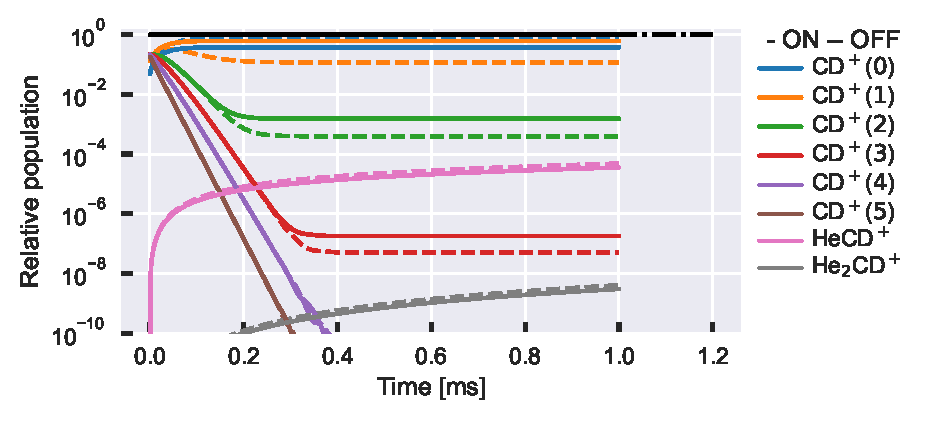
\includegraphics[width=1\textwidth]{figures/simulations/coll_rad_att/CD+_He_f-time__transition_0-1_0.001s_population_ratio.pdf}}{}{\label{fig:thz-sim:rel-pop:1ms}}
    \hfill
    
    \Subfigure[0.5]{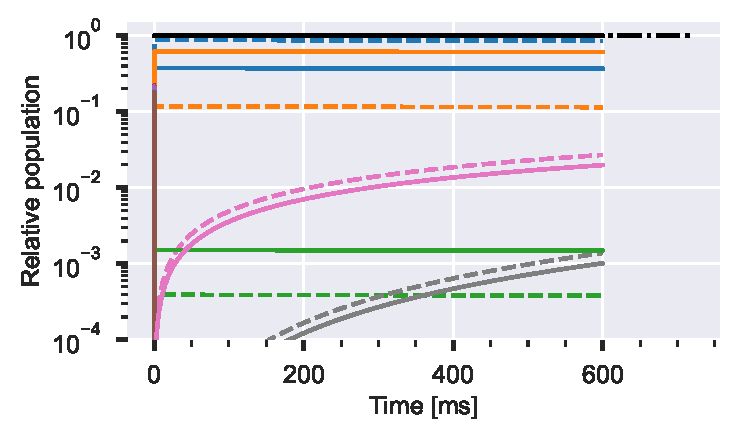
\includegraphics[width=1\textwidth]{figures/simulations/coll_rad_att/CD+_He_f-time__transition_0-1_0.6s_population_ratio.pdf}}{}{\label{fig:thz-sim:rel-pop:0.6s}}
    \hfill
    \Subfigure[0.45]{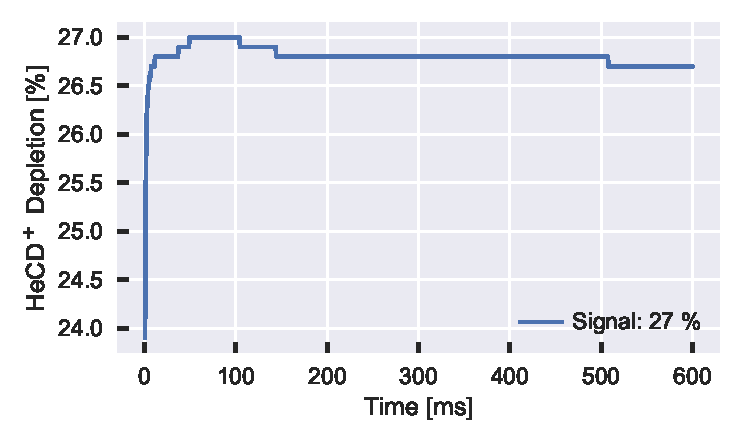
\includegraphics[width=1\textwidth]{figures/simulations/coll_rad_att/CD+_He_f-time__transition_0-1_0.6s_signal.pdf}}{}{\label{fig:thz-sim:signal:0.6s}}
    \hfill
    
    \Subfigure[0.5]{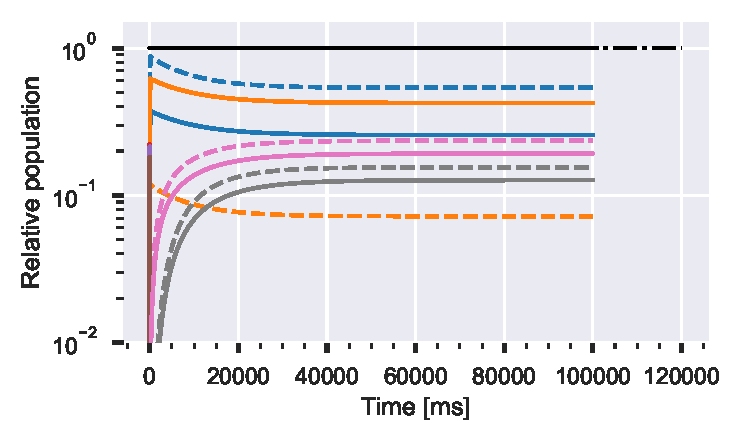
\includegraphics[width=1\textwidth]{figures/simulations/coll_rad_att/CD+_He_f-time__transition_0-1_100.0s_population_ratio.pdf}}{}{\label{fig:thz-sim:rel-pop:100s}}
    \hfill
    \Subfigure[0.45]{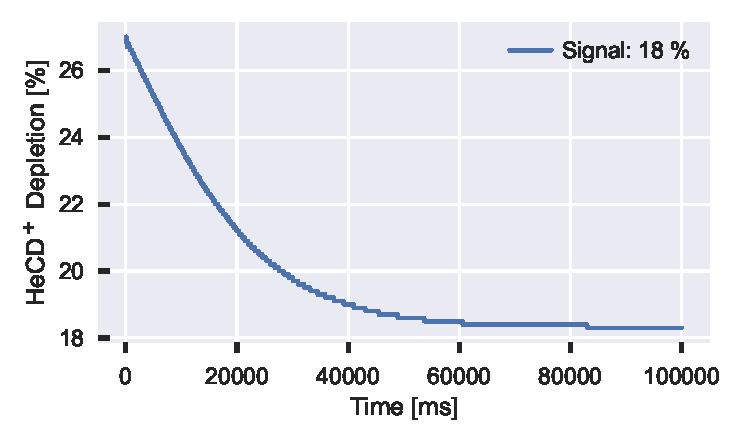
\includegraphics[width=1\textwidth]{figures/simulations/coll_rad_att/CD+_He_f-time__transition_0-1_100.0s_signal.pdf}}{}{\label{fig:thz-sim:signal:100s}}
    \hfill
    
    \end{adjustbox}
    
    \caption{
        (a) Simulated relative rotational level populations for
        \CD and corresponding numberof He$_n$\CD clusters (n=1, 2) 
        where \CD$(J)$ indicates \CD in $J$ rotational state. 
        The simulation conditions are as follows: $k_{3_1}$ ratio, $a=0.5$, 
        collisional rates for T$_{coll}=7$ K  (at $t=0$, T$_{coll}=300$ K), 
        Helium number density $2.2 \cdot 10^{14}$ \percc and radiation power $3.5\cdot10^{-5}$ W. 
        The solid and dashed lines correspond to, with (-ON) and without (--OFF), 
        the presence of radiation on the \CD \CDline transition frequency. 
        The simulation duration for (a) 1 ms, (b) 600 ms and (d) 100 s. 
        Figures (c) and (e) correspond to signal intensity, i.e., He\CD depletion \% as a 
        function of time for (b) and (d), respectively. 
        At longer time the signal decreases because of the competing processes at different timescale (faster radiative and collision; and slow complex formation rates) and eventually reaches an equilibrium value.
    }
    
    \label{fig:thz-sim:rel-pop}

\end{figure}


The attachment and dissociation rate timescale are in the order of $10^{-1}$
\pers\ (see Table \ref{appendix:tab:attachment-rate-coefficients}). Thus, the
population of the first complex (He\CD) is very small, i.e., $<10^{-4}$ in relative
population, during the first 1 ms; however, it tends to increase. Therefore,
when the simulation is extended for a longer duration, i.e., for 600 ms (see
Figure \ref{fig:thz-sim:rel-pop:0.6s}) and 100 s (see Figure
\ref{fig:thz-sim:rel-pop:100s}), the He\CD relative population reaches 0.03 and
attains equilibrium at 0.2 after 40 s, respectively. Also, regarding our initial
consideration of a 2-level quantum system, the figures
support this assumption, i.e., at 7 K temperature and $t=0.6$ s duration, 
the relative population pumped into \CD(0)$=0.86$ and \CD(1)$=0.11$ 
but for \CD$(J\geq 2)$ it is $\ll 10^{-4}$.

As expected, and shown in Figure \ref{fig:thz-sim:rel-pop:0.6s} and
\ref{fig:thz-sim:rel-pop:100s}, a significant difference in population is
observed in the first He\CD complex with (-ON) and without (-\--OFF) radiation resonant 
with the \CDline transition of \CD. This difference is indeed the measured ROSAA 
depletion signal of He\CD at resonance. Figure \ref{fig:thz-sim:signal:0.6s} represent 
the expected signal intensity of the measured rotational spectrum (as shown in Figure \ref{fig:thz}) 
for a trap duration of 600 ms.

At longer time (100 s duration) the signal decreases (see Figure \ref{fig:thz-sim:signal:100s}),
this maybe be due to the fact that the formed higher order of complexes 
does not contribute to the signal intensity and subsequently causes the signal to decrease, 
eventually reaching a equilibrium value. 
Before analysing further, let us look at approaches to validate our model.


There are three direct ways to verify the validity of the numerical model.

\begin{enumerate}
    \item  One is to compare it with the Boltzmann distribution when only collisional
          processes are considered. Then at equilibrium, the relative population of
          \CD$(J)$ reaches T$_{coll}$, which should be equivalent to the
          Boltzmann distribution at T$_{coll}$. This has been discussed in Section
          \ref{subsec:CD+-kinetics-simulation-coll} and can be verified in Figure
          \ref{fig:ROSAA-sim-collisional-boltzmann}.
    \item Another way is when collisional and radiative processes are involved,
          competing with each other. Under conditions when the radiative process (for
          the \CDline transition of \CD) dominates the collisional process (Coll. $\ll$
          Rad.), the equilibrium relative population of \CD$(J=0)$ and \CD$(J=1)$ should
          reach their statistical weights ($g(J) = 2J+1$), i.e., 0.25 and 0.75,
          respectively. This has been discussed in section
          \ref{subsec:CD+-kinetics-simulation-coll-rad} and can be verified in Figure
          \ref{fig:ROSAA-sim-coll-rad-boltzmann-higher-rad}.
    \item Another direct approach is to verify the the signal intensity is $\sim 0$ when
          the $k_{3_1}$ ratio $a=1$. This indicates that the rate constants are not
          state-dependent but rather the same, thus leading to the absence of ROSAA
          signal intensity.
\end{enumerate}

In addition to validating the third point (3) for the numerical model, similar
to the signal intensity plot as shown in Figure \ref{fig:thz-sim:signal:0.6s}
and \ref{fig:thz-sim:signal:100s}, a complete overview of signal intensity
simulations as a function of power ranging from $10^{-7}-10^{-2}$ W, number
density from $10^{12}-10^{16}$ \percc and $k_{3_1}$ ratio $a$ ranging from
$0.3-1$, is shown in Figure \ref{fig:thz:all-simulation}. The third point can
be verified in Figure \ref{fig:thz:all-simulation:0.1a}, where the
signal intensity is 0 as expected when $a=1$.\\

\begin{figure}[!htb]
    \centering
    
    \Subfigure[0.3]{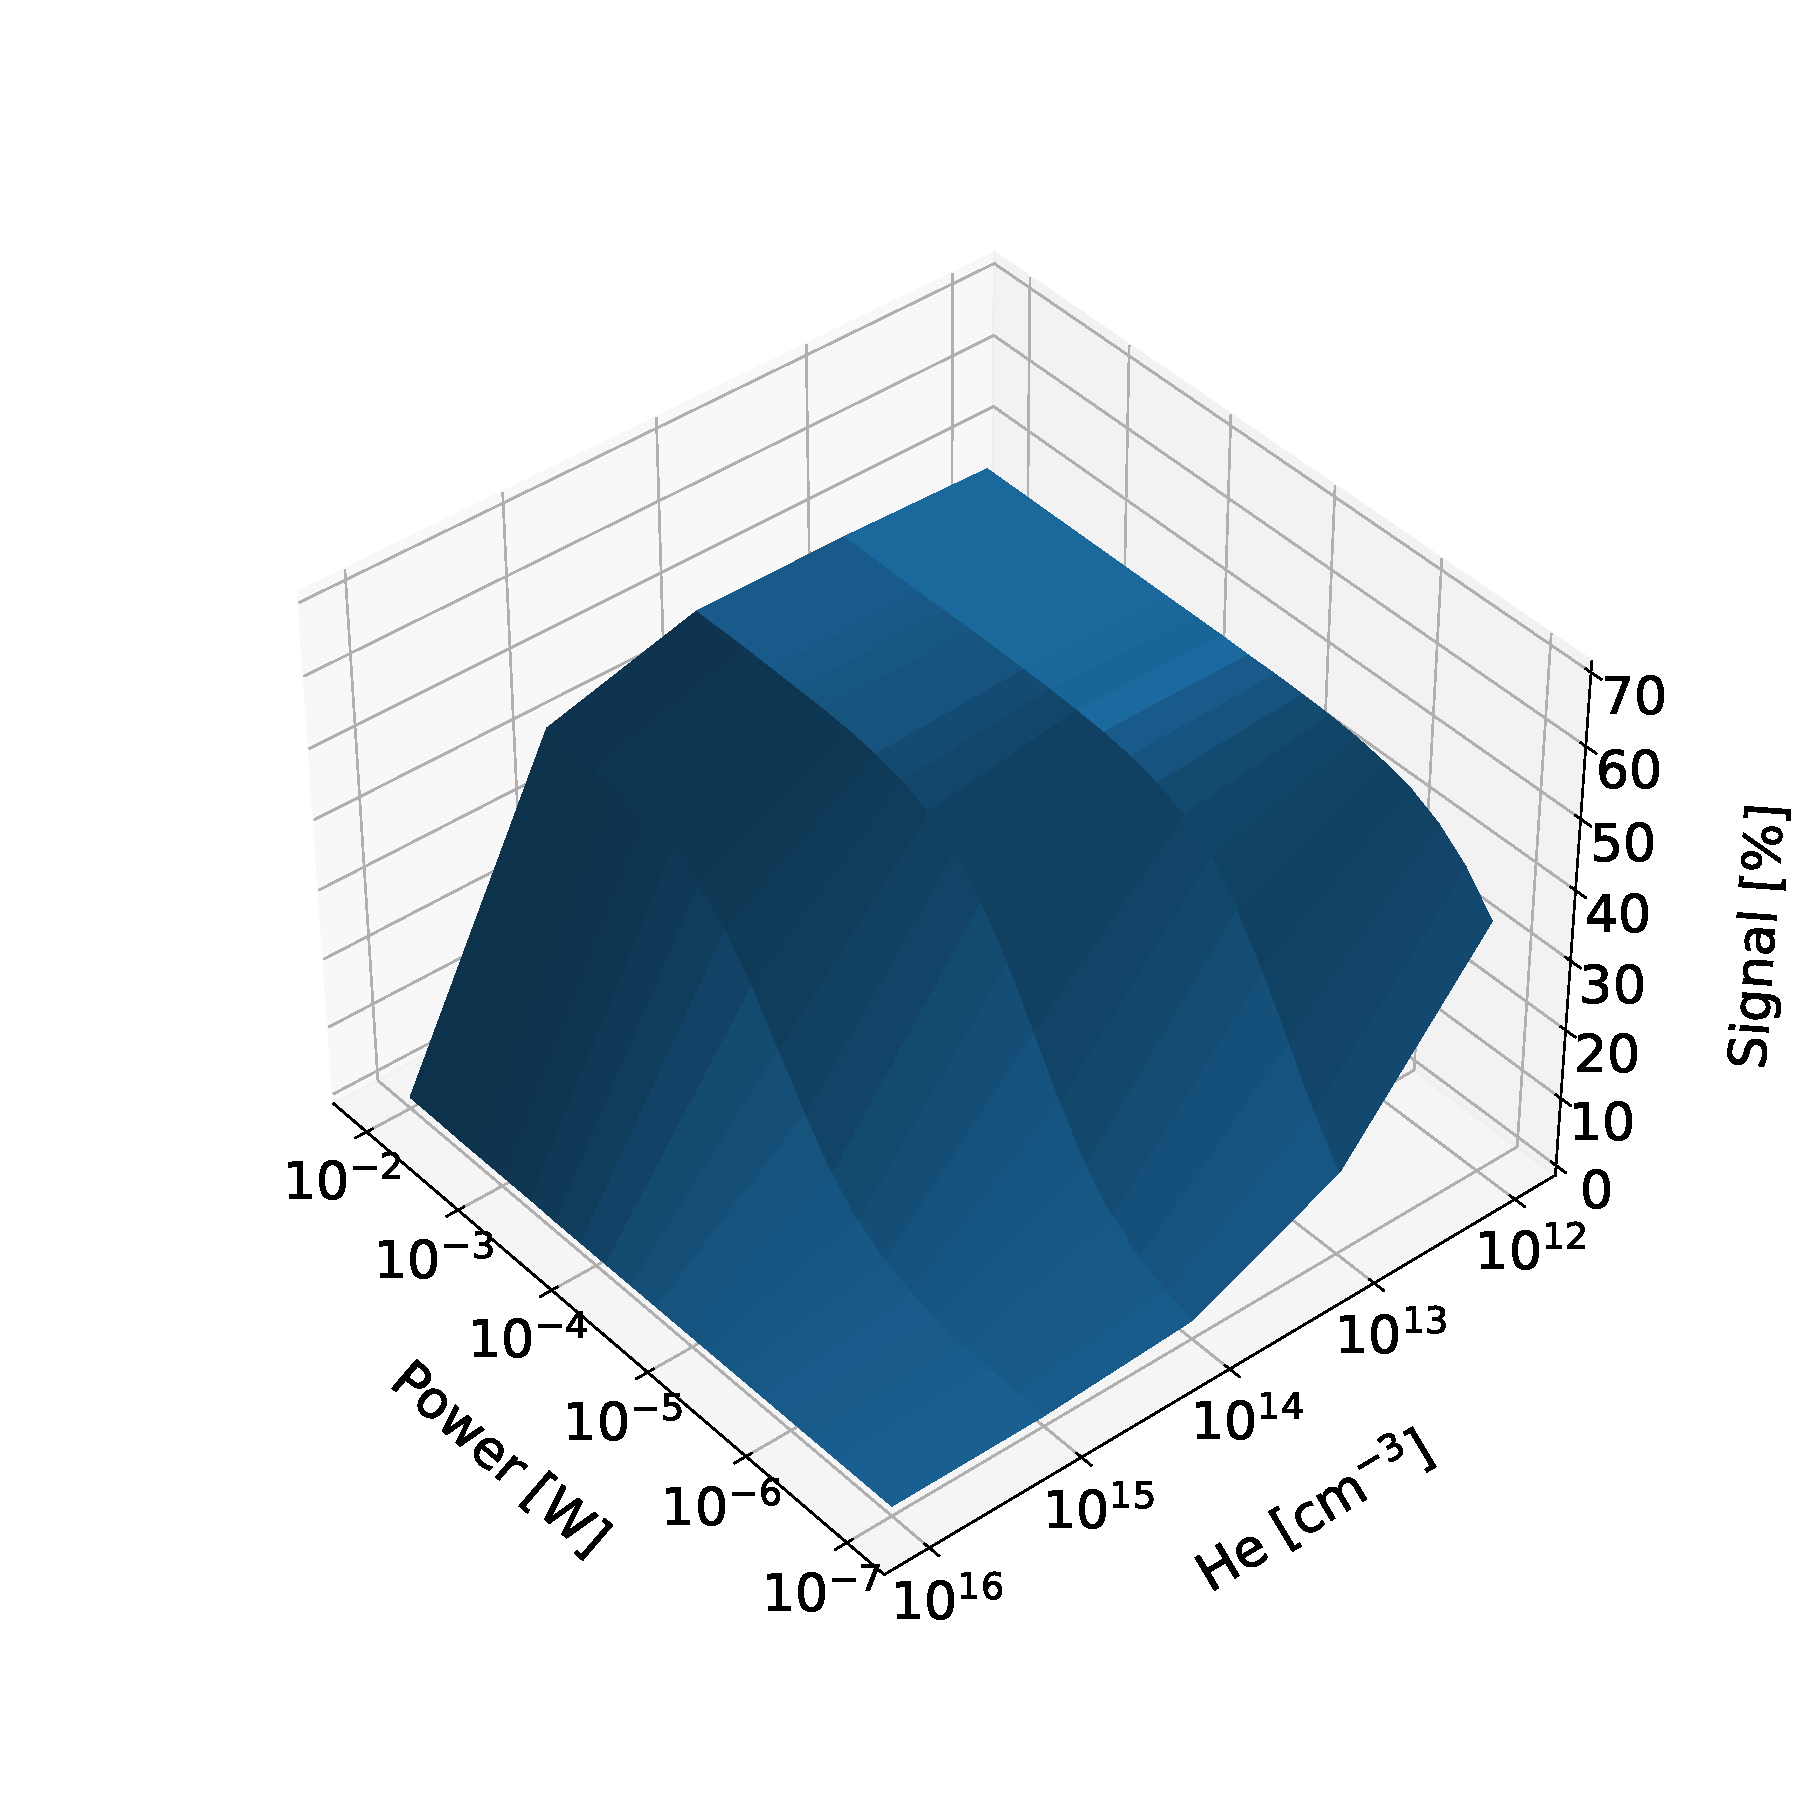
\includegraphics[width=1\textwidth]{figures/simulations/ROSAA/f-power_1e-7-1e-2/k3_branch_0.30.pdf}}{$k_{3_1}$ ratio $=0.3$}{}
    \hfill
    \Subfigure[0.3]{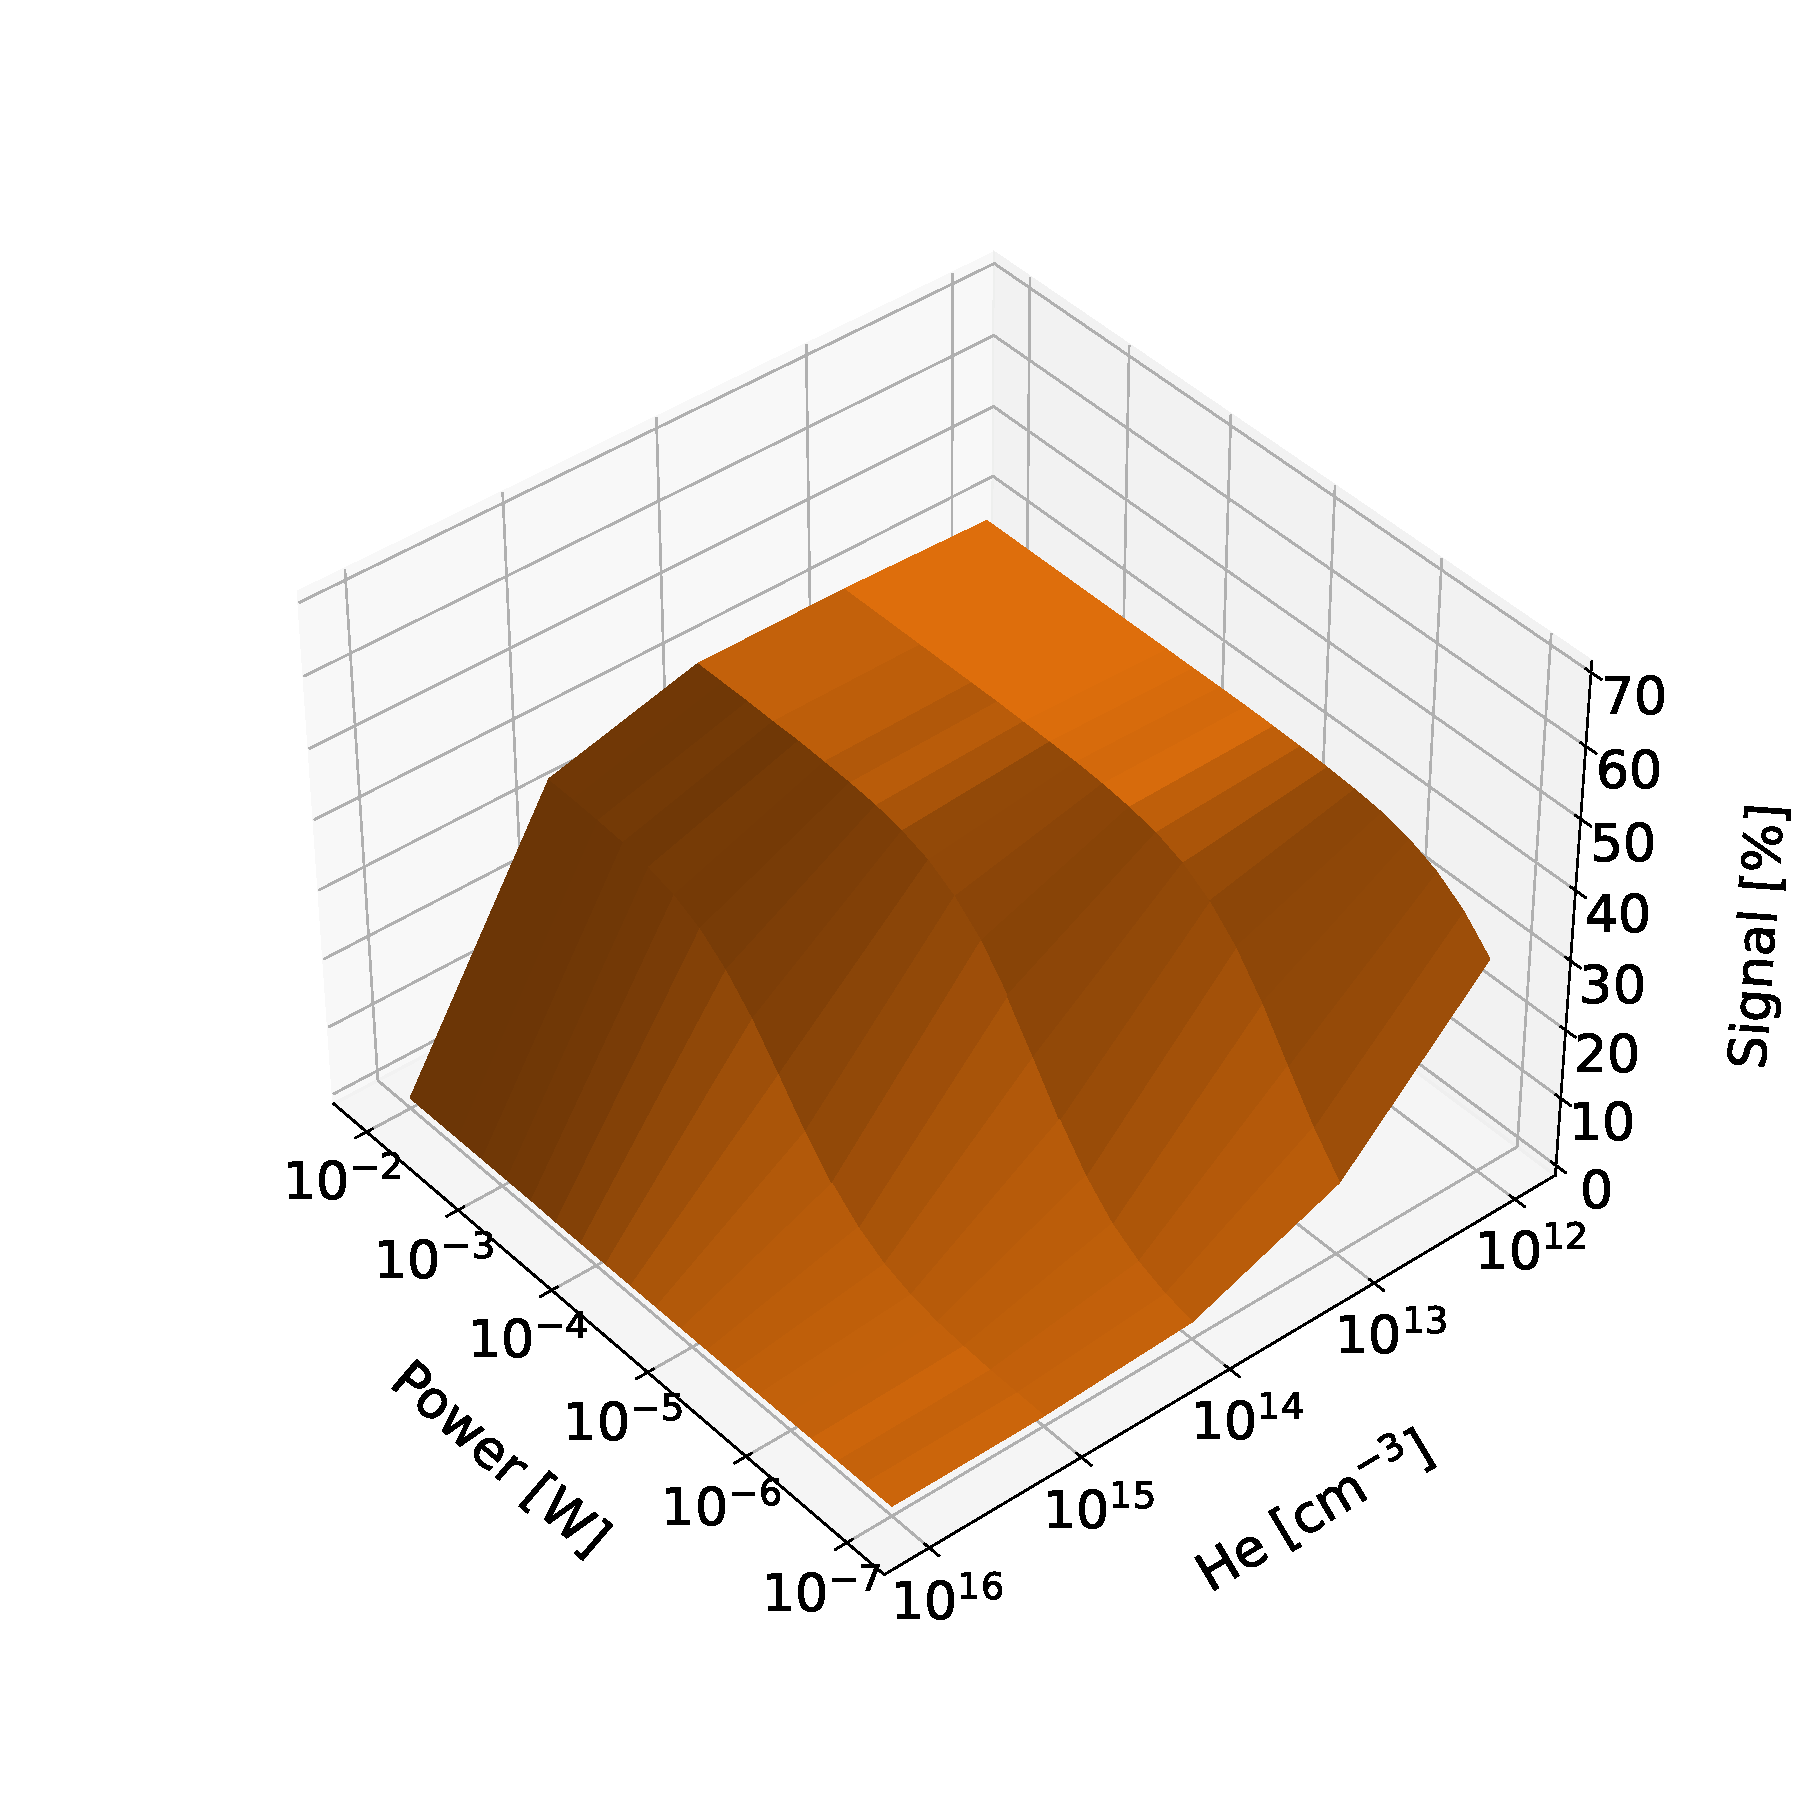
\includegraphics[width=1\textwidth]{figures/simulations/ROSAA/f-power_1e-7-1e-2/k3_branch_0.40.pdf}}{$k_{3_1}$ ratio $=0.4$}{}
    \hfill
    \Subfigure[0.3]{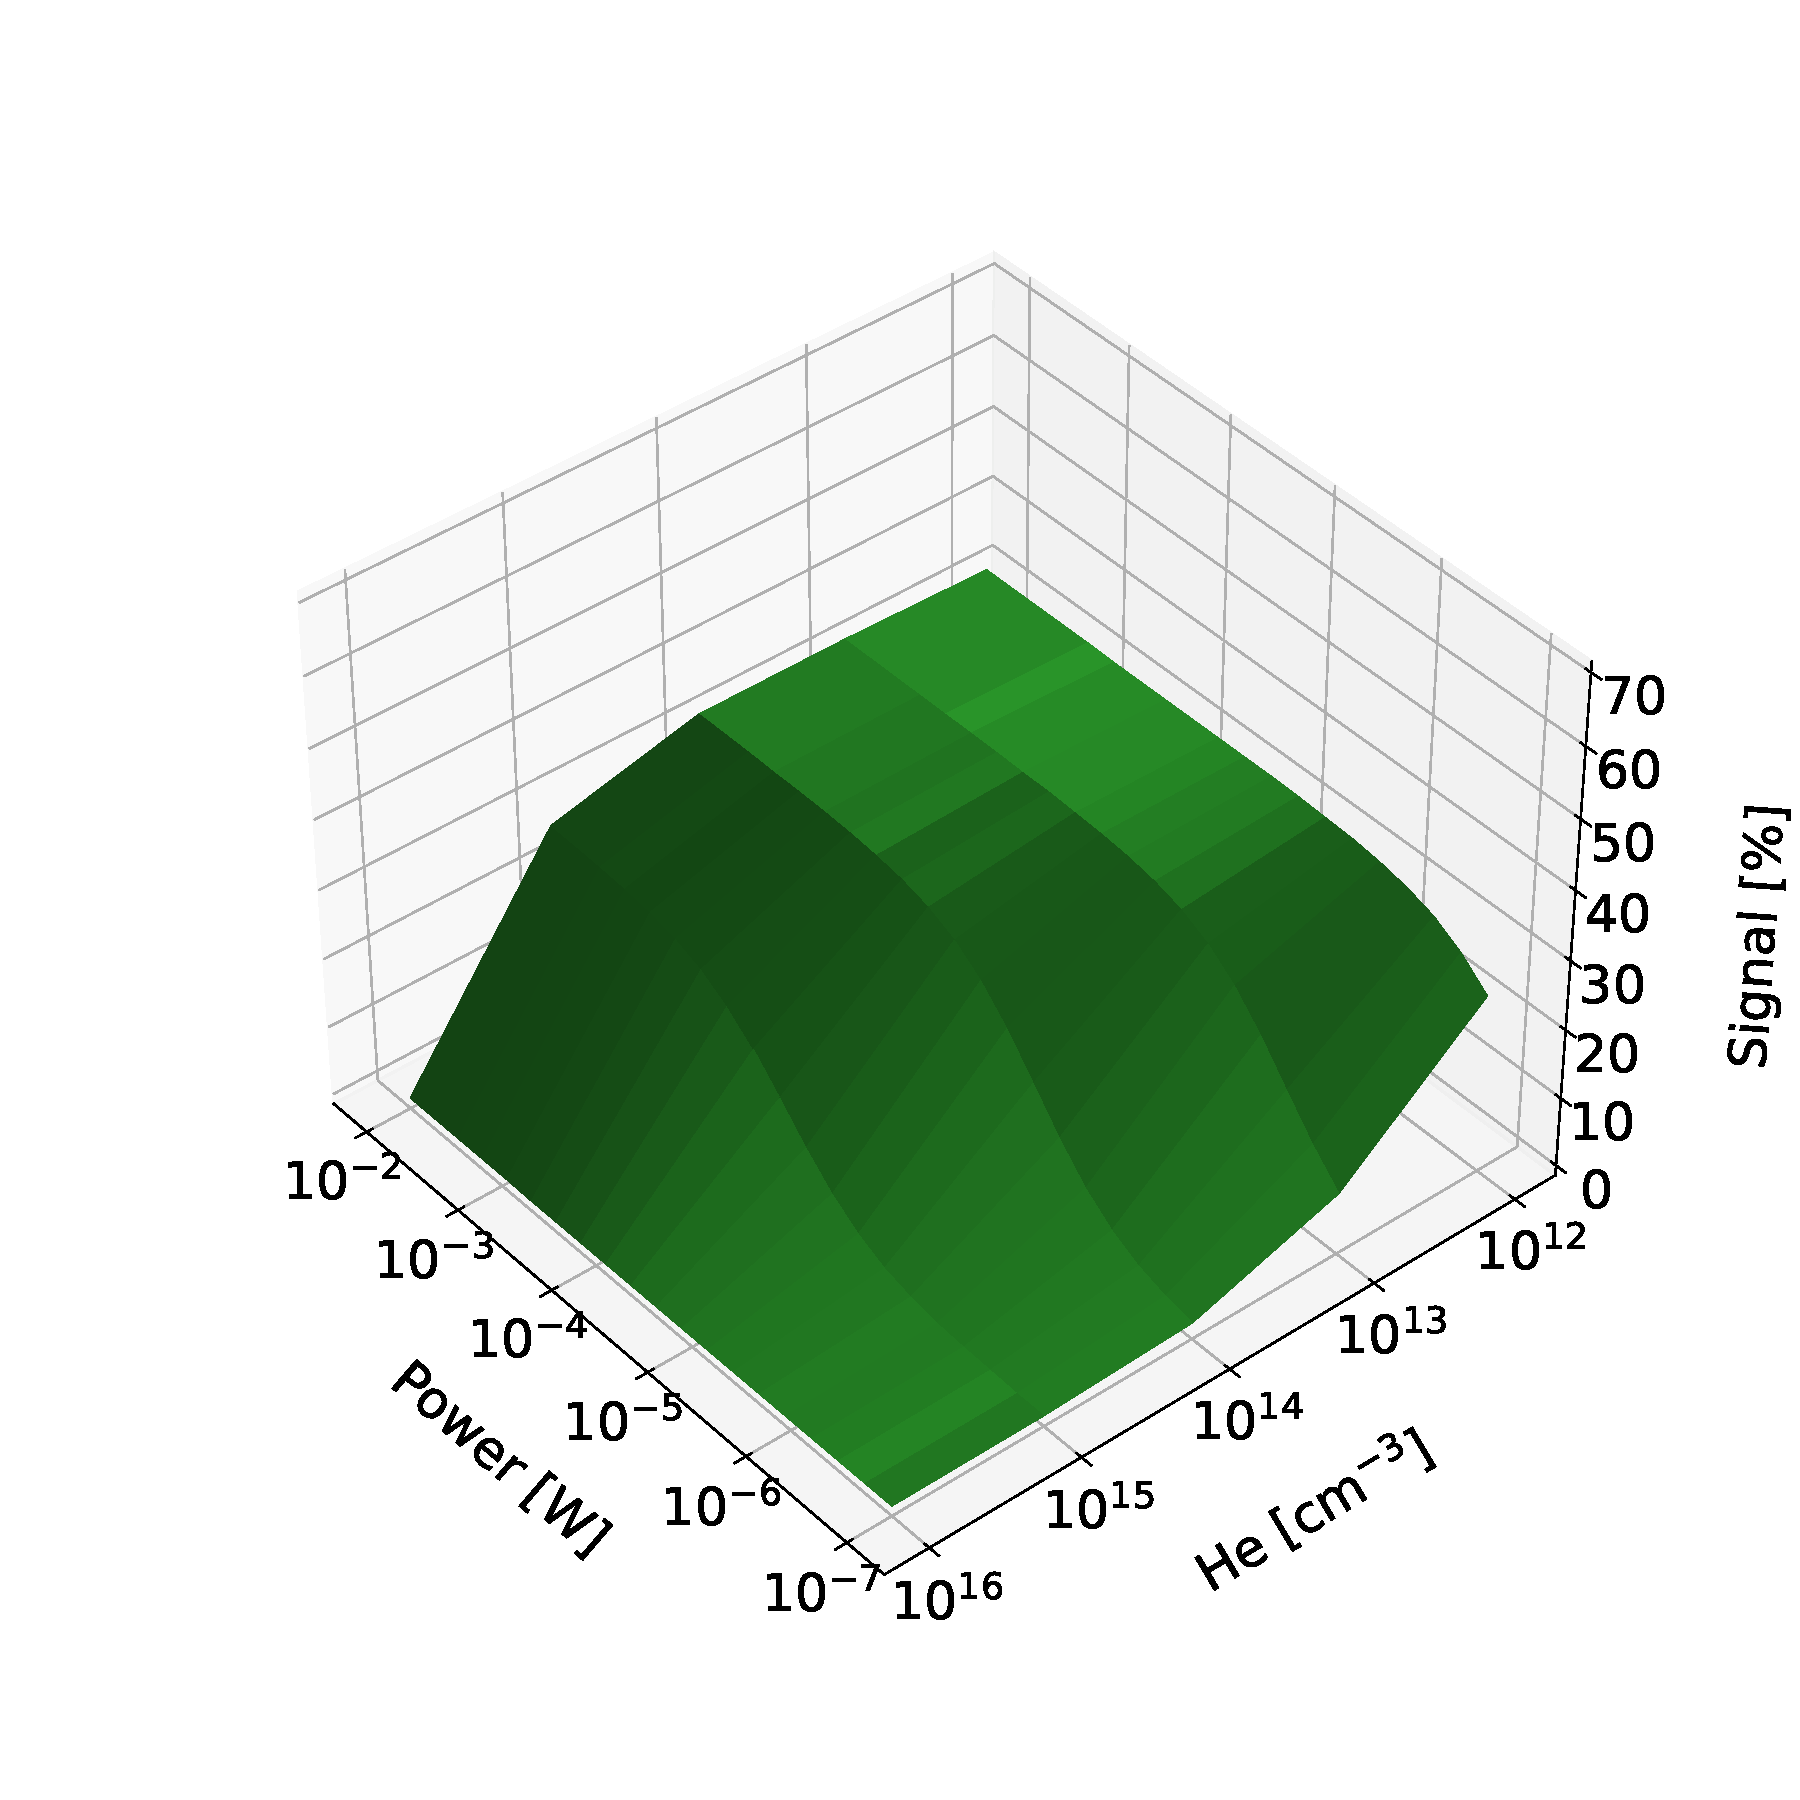
\includegraphics[width=1\textwidth]{figures/simulations/ROSAA/f-power_1e-7-1e-2/k3_branch_0.50.pdf}}{$k_{3_1}$ ratio $=0.5$}{\label{fig:thz:all-simulation:0.5a}}
    \hfill
    \Subfigure[0.3]{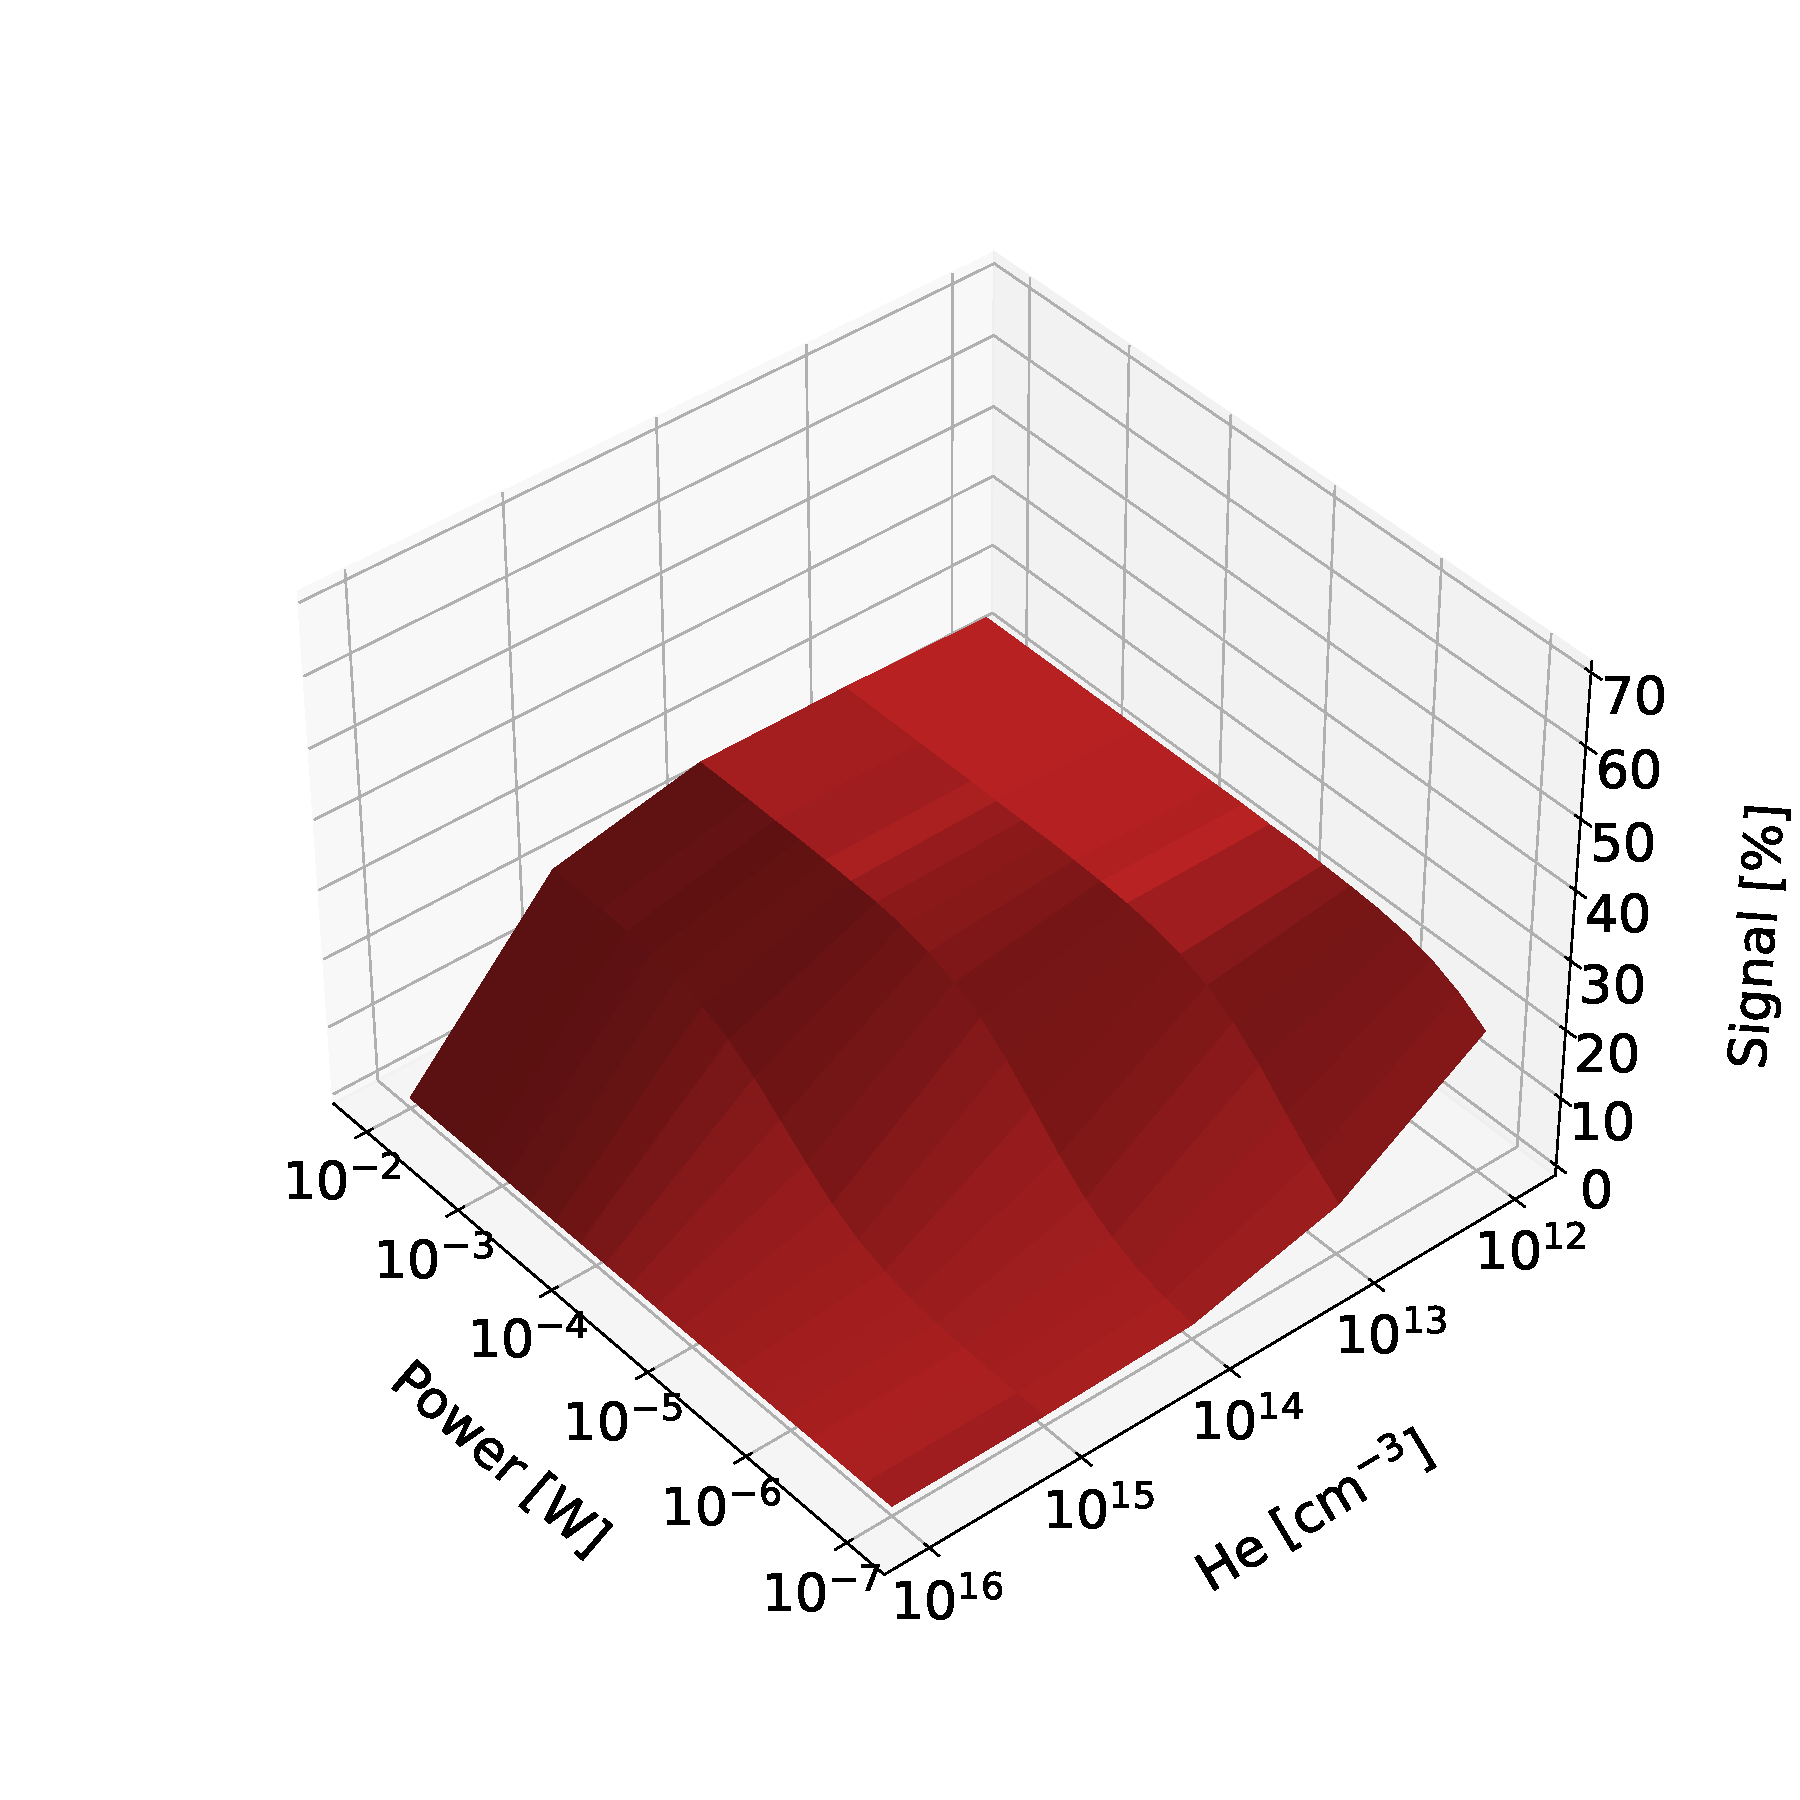
\includegraphics[width=1\textwidth]{figures/simulations/ROSAA/f-power_1e-7-1e-2/k3_branch_0.60.pdf}}{$k_{3_1}$ ratio $=0.6$}{}
    \hfill
    \Subfigure[0.3]{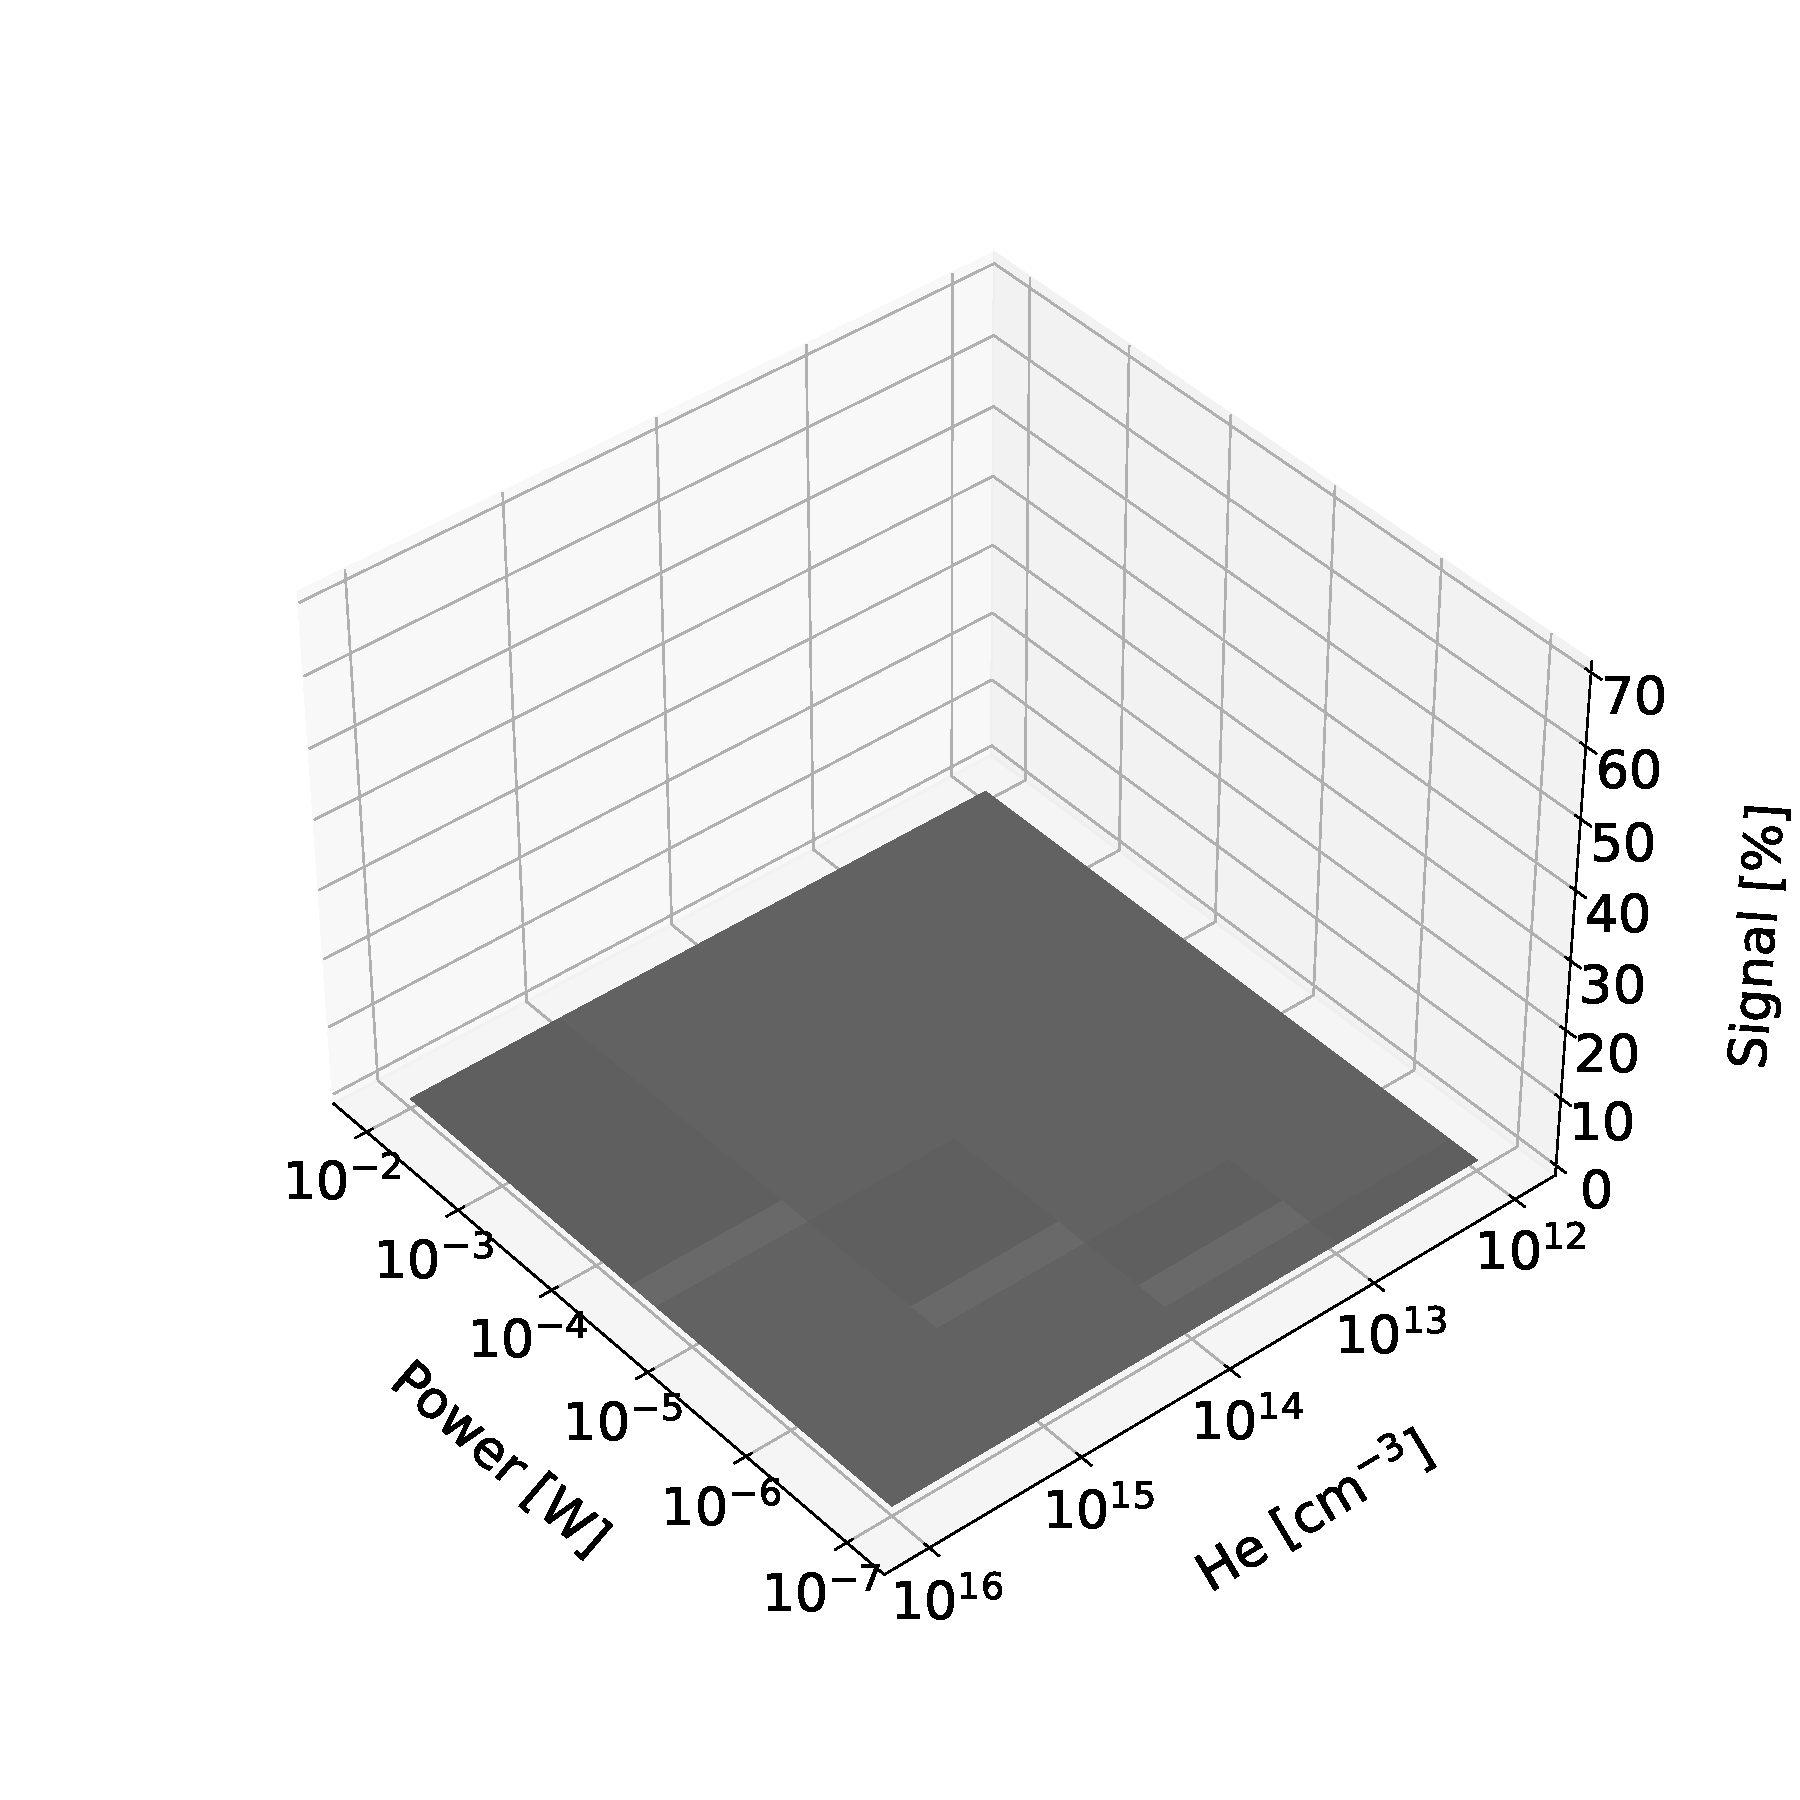
\includegraphics[width=1\textwidth]{figures/simulations/ROSAA/f-power_1e-7-1e-2/k3_branch_1.00.pdf}}{$k_{3_1}$ ratio $=1$}{\label{fig:thz:all-simulation:0.1a}}
    \hfill
    \Subfigure[0.3]{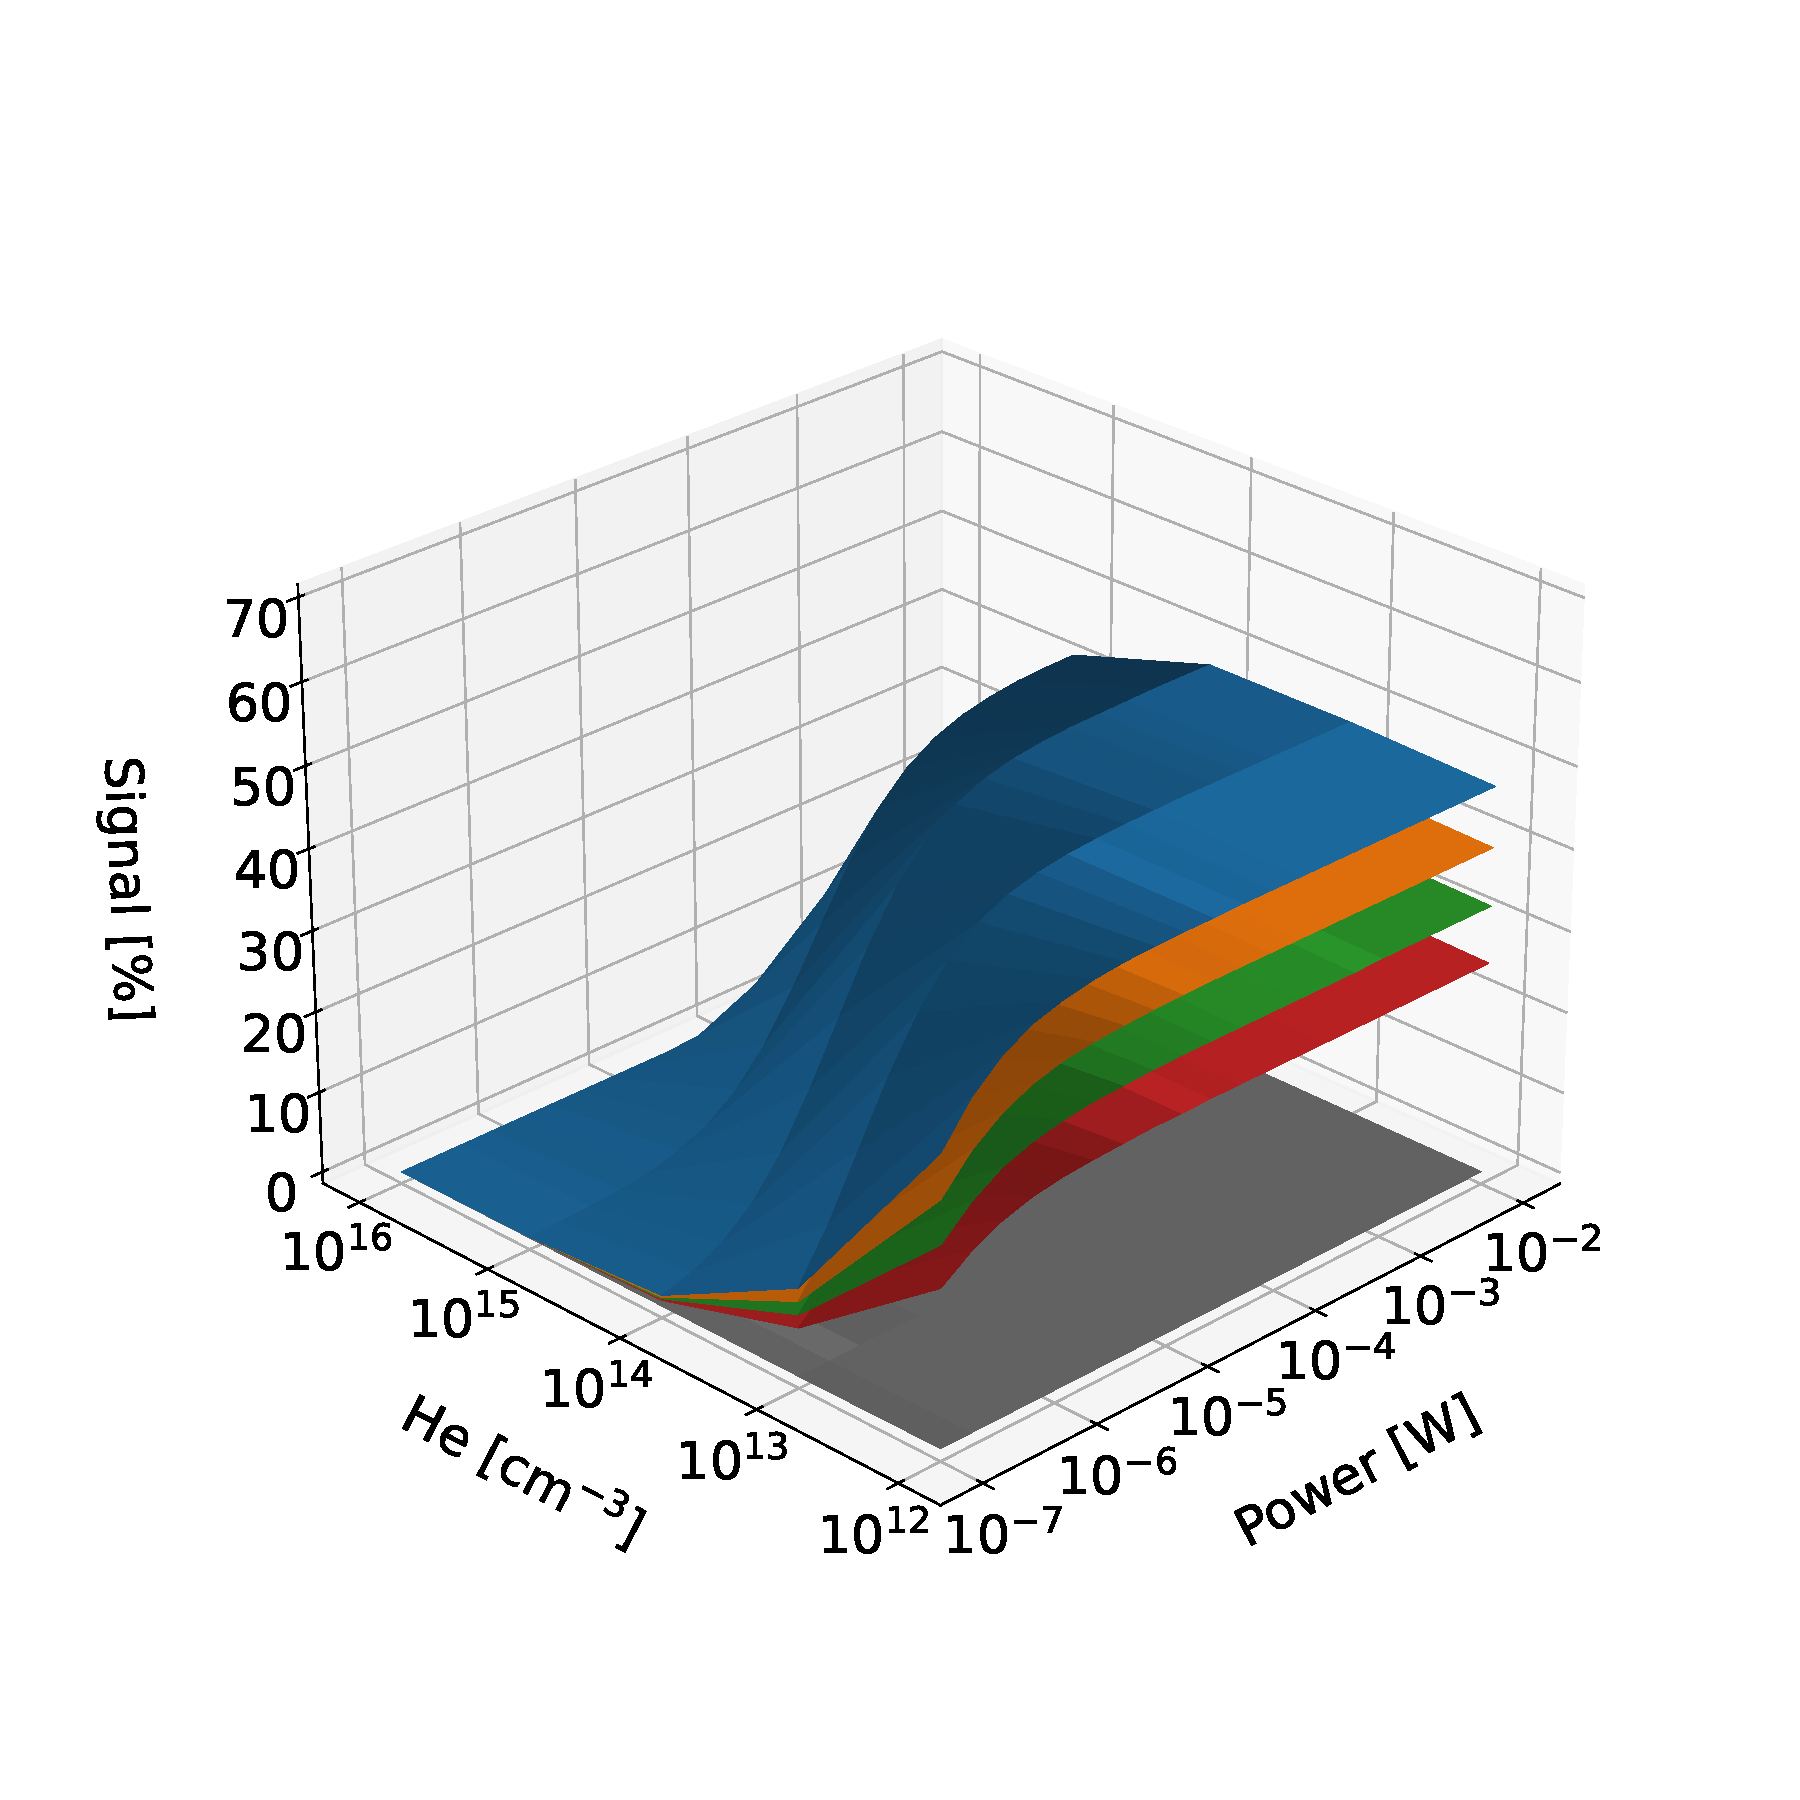
\includegraphics[width=1\textwidth]{figures/simulations/ROSAA/f-power_1e-7-1e-2/combined.pdf}}{combined}{}
    
    \caption{Numerical simulation of ROSAA process with computed signal intensities as a function of radiation power, $10^{-7} - 10^{-2}$ W, He number density, $10^{12} - 10^{16}$ \percc, and $k_{3_1}$ ratio, $0.3-1$, at 600 ms trap duration and T$_{coll}=7(1)$ K temperature. The captions of subplots (a)-(e) indicate the respective $k_{3_1}$ ratio value. (f) as captioned, shows the combined plots of (a)-(e).}
    \label{fig:thz:all-simulation}
\end{figure}

% \textbf{Comparing to ROSAA experiment:}\\
The experimental ROSAA signal strength under the condition of $2.2 \cdot 10^{14}$
\percc\ helium number density and $35\ \mu$W power at 600 ms trap time is
$26(1)$\% (see Table \ref{tab:CD+_He}). With the same condition, Figure
\ref{fig:thz-sim:signal:0.6s} predicts a signal intensity of 27\% at $t=600$ ms.
Therefore, there is close agreement with our numerical model simulation
results. Figure \ref{fig:thz:all-simulation:0.5a} depicts an overview of the
achievable signal intensity as a function of number density and power for $a=0.5$
and 600 ms duration. They are directly proportional to radiation power and are
inversely proportional to number density. We have utilised our THz radiation
source to full power without attenuation (see Section
\ref{subsec:ir:radiation-source}), with the number density adjusted for
$700-1000$ counts of He\CD complexes formed for spectroscopy measurement (see
Figure \ref{fig:masspec}). As shown in Table \ref{tab:CD+_He}, we have measured
at different number densities, and $2.2 \cdot 10^{14}$ \percc\ at
T$_{trap}=$4.8(3) K (T$_{coll}=$7(1) K) appears to be an optimal condition to
achieve a signal of $27(1) \%$ which is not far from the maximum achievable
signal, i.e., $\approx 33 \%$ as shown in Figure
\ref{fig:thz:all-simulation:0.5a}.

The Ne-ROSAA measurement is shown in Figure \ref{fig:thz:NeCD+} and Table
\ref{tab:CD+_Ne}. Since a pure Ne kinetics measurement of the attachment process was very challenging at
low temperatures due to freeze-out , it will be explored in detail in future
studies, and here we assume the same attachment and dissociation rate
coefficients as for helium. We run simulations under the following conditions:

\begin{align*}
    [Ne]            & = 1.5 \cdot 10^{14} \text{ cm}^{-3} \\
    P               & = 35\ \mu \text{W}                  \\
    t               & = 600 \text{ ms}                    \\
    \text{T}_{trap} & = 8.7 \text{ K}                     \\
    \text{T}_{coll} & = 18.2 \text{ K}                    \\
\end{align*}

The experimentally measured Ne-ROSAA signal of $24(1) \%$ fits with the
simulation result ($24 \%$) but only with a reduced $a=0.25$ rather than $a=0.5$,
at T$_{coll}=18.2$ K. As also discussed in \citet{Brunken2017}, $k_{3_1}(J=1)$
likely shows a steeper decreasing temperature dependence than $k_{3_1}(j=0)$.\\

Our initial goal was to develop an adaptable and robust numerical
simulation model (with an easy-to-use graphical user interface). In addition to
investigating the He-\CD and Ne-\CD ROSAA model, it can be easily extended to investigate the
CO$^+$ molecular ion (Chapter \ref{chapter:CO+}), which is an open-shell
species hence the rotational quantum states split into fine structure levels
due to non-zero net electron spin. Therefore, we have shown that extending this
model to different systems is possible and will be used to predict the ROSAA
signal intensity for rotational transition measurements when energy level
information (from the calculation) and rate coefficients from kinetic
measurements are available.

The next section briefly discusses an interesting observation on the
temperature dependence of ternary attachment rate coefficients.

% \clearpage
